% 第四章 内务府的人
% 原书页码：111；标题
\section{内务府的人}
\par
% 原书页码：111–112；段落（跨页续段）
南怀仁去世后四年，传教士终于实现了他们人华百年来的目标：%
天主教得到了朝廷认可，合法地位得到了正式确认。1692年，经过索%
额图多方打点、私下运作，礼部最终同意了天主教的传播。康熙在礼%
部部议基础上下发了容教诏书。根据当时法国传教士洪若翰的记录，%
传教士协助大清签订了与俄罗斯的条约后，康熙私下授意他身边的传%
教士徐日升和安多，让他们在公开上朝的时候，上一个折子来请求允%
准天主教的传播。据洪若翰提供的细节，康熙在朝堂上收到传教士的%
折子以后，假装什么都不知道，把这份折子和其他收到的折子混在一%
起，交给了内阁官员，由他们将折子下放到朝廷相应部门处理。礼部%
收到这份折子，部议后，否决了请求。康熙收到礼部否决意见后，并%
没有做出反应。洪若翰解释，因为康熙也得尊重朝廷部门的意见，不%
好公开提出异议。这样私下运作的任务就落到了索额图身上。\NoteRef{4}{1}三年%
前传教士帮他跟俄罗斯谈判时，索额图就许诺过要回报传教士。\NoteRef{4}{2}索额%
图具体是如何操办的，传教士没有记录。不过在索额图私下运作以后，%
礼部尚书顾八代给出了允许天主教传播的意见：%
\par
% 原书页码：112；段落
{\bookkai 臣等会议得，查得西洋人仰慕圣化，由万里航海而来。现今治理}%
{\bookkai 历法，用兵之际，力造军器火炮；差阿罗素\AuthorNote{〔俄罗斯〕}，诚心效力，克}%
{\bookkai 成其事，劳绩甚多。各有居住西洋人，并无为恶作乱之处。又并非左}%
{\bookkai 道惑众，异端生事。喇嘛僧道等寺庙尚容人烧香行走，西洋人并无违}%
{\bookkai 法之事，及行禁止，似属不宜。相应将各处天主堂俱照旧存留，凡进}%
{\bookkai 香供奉之人，仍许照常行走，不必禁止。俟命下之日，随行直隶各省}%
{\bookkai 可也。\NoteRef{4}{3}3}%
\par
% 原书页码：112；段落
传教士在天文历法、制造火器以及与俄罗斯谈判这三条公认的功绩是%
容教的基础。而这三条功绩中，天文历法、制造火器都是南怀仁的功%
劳，这两条也刻在了南怀仁的墓碑上。与俄罗斯的最后边境谈判虽然%
发生在南怀仁死后一年，但前面数十年的准备工作都是南怀仁一手操%
持的。%
\par
% 原书页码：112；段落
顾八代给出的容教理由，在逻辑上其实很直白，就是既然其他外%
来宗教都允准在华传播，那么天主教也应该被容许。这个容教诏书印%
证了耶稣会传教士长久以来的策略判断，就是在北京朝廷内的服务有%
可能为整个在华传教打开方便之门。康熙在收到礼部建议后第三天就%
发了容教诏书。这一消息也迅速传回了欧洲，一下激起了更多传教士%
来华传教的热情。在1701年，也就是容教诏书颁布十年以后，整个%
来华的传教士人数，以及天主教受洗人数都成倍增长。\NoteRef{4}{4}%
% 原书页码：113；标题
\subsection{臣子和奴才}
\par
% 原书页码：113；段落
南怀仁是康熙的老师，也是康熙年轻时身边的重要人物。在清代%
历史中，围绕南怀仁以及后来在康熙身边的传教士一直有一个问题：%
他们在宫中行走的身份到底是什么？我们都知道，出入紫禁城从来不%
是件容易的事，更不要说像北京耶稣会士那样日常出现在皇帝身边。%
教康熙中国历史以及各种儒家经典的老师，都有各种朝廷头衔，皇帝%
的课业安排也都是由礼部承办。南怀仁尽管也在钦天监任职，但这职%
位并不能让他经常接触到皇帝；而且后来入宫教康熙的传教士，比如%
张诚、白晋等人，连在钦天监的职位都没有。所以这些传教士究竟是%
以何种身份在宫中行走?%
\par
% 原书页码：113–114；段落（跨页续段）
所谓身份问题，按古代的说法就是名分问题。大部分传教士都没%
有朝廷官位。也就是说他们和康熙没有君臣名分。但传教士在康熙身%
边行走是人所共知的，那他们是以什么名分出现在皇帝身边的？这个%
问题其实涉及明清体制中的一个重大区别，就是清朝治下，除了君臣%
名分以外，还有一个主奴名分存在。按中国传统政治理论，“普天之%
下，莫非王土；率土之滨，莫非王臣”。也就是说，皇帝和他的臣子%
只有一个名分，就是君臣名分。清朝入京后沿用明制，自然也就沿用%
了明代朝廷制度下的君臣关系。在清朝八旗之内，满人的主奴关系还%
保留沿用。也就是说，清朝治下，皇帝和他的臣子有君臣和主奴两种%
名分存在。所以我们能看到清朝的大臣，给皇帝上书，有些自称奴才，%
有些自称臣。还有一些人既是皇帝的奴才又是皇帝的大臣，两种身份%
并存。比如曹寅，他给康熙的同样一份奏折中，会时而自称臣时而又%
自称奴才。%
\par
% 原书页码：114；段落
在满人人关以前，主奴关系是满人游牧传统中军事等级关系和%
社会等级关系的基础。\NoteRef{4}{5}东北地广人稀，满人也深知奴隶是重要的经%
济资源。因而他们推崇主奴之间以家为纽带，和睦相处。\NoteRef{4}{6}奴才身份是%
世袭的，就算由于某些原因，奴才的奴籍被去除了，但他们的后人与%
原来主子之间的主奴派系源流关系依然存在。\NoteRef{4}{7}%
\par
% 原书页码：114；段落
满人社会中的奴才和汉人社会中的“奴”是不一样的。汉人社%
会的“奴”属于贱民阶层，地位在贵族、官吏、平民之下。“奴”和%
其他属于贱民阶层的人，比如乐户、娼妓之类，社会地位低，多方%
面受歧视，而且法律和社会习俗还对贱民阶层有很多专门的行为约%
束，比如良贱不能通婚等。\NoteRef{4}{8}但在满人社会，奴才的身份并不代表一%
个人社会地位低，他们社会地位的高低主要取决于其主子的社会地%
位。满人中大量高官就是奴才出身。因此，满人的奴才身份不直接%
代表其社会阶层，而主要是为了说明此人和其主子之间的主奴关系，%
以及相关的派系源流。%
\par
% 原书页码：114；段落
满人靠征战起家，最初也没有科举制度。他们的人力资源选拔是%
以家庭为中心来建立的。他们的关系网中最重要的是血缘关系，其次%
是从血缘关系衍生出来的婚姻关系。随着清朝势力17世纪的急剧扩%
张，血缘关系和婚姻关系不能为清朝提供足够的人力资源。这种情况%
下，家庭框架下的主奴关系就变得十分重要。%
\par
% 原书页码：115；段落
各种书籍中经常出现的包衣奴才就是奴才的一种。一个清朝权%
贵，挂在名下的奴才成百上千，但真正在身边伺候的那些奴才才是包%
衣奴才。包衣奴才基本就是家奴的意思。大约在满人1644年人京以%
后，包衣奴才就用来专指皇帝和皇亲国戚家的奴才了。皇帝的包衣奴%
才众多，管理这些包衣奴才的机构是内务府。%
\par
% 原书页码：115；段落
内务府是满人人京前就有的机构。入京以后，顺治年间，内务府%
还和宫内的太监机构并立于宫中，分工管理皇帝的宫内事务。在鳌拜%
时期，为了避免明代宦官专权再次发生，清朝裁撤了宫内太监机构，%
把太监并入内务府中，由内务府管理。后来清宫历史、小说等提到太%
监就会提到内务府，就是这个原因。但需要强调的是，管理太监并不%
是内务府的主业，其主要职能是管理皇帝的包衣奴才。%
\par
% 原书页码：115；段落
从机构运作来看，内务府不是国家官僚系统的一部分。因为它从%
诞生起到后来的实际运作，都是用来帮助皇帝打理家庭和个人私事%
的。\NoteRef{4}{9}内务府独立运作于国家官僚系统外，也就是说不受朝廷各部门的%
管辖。内务府不仅在北京管理运作宫中的日常事务，它还有一个延伸%
到各个地方的内部网络。内务府中皇帝的小金库，是和户部管理的国%
库分开的。\NoteRef{4}{10}它的资金来源包括土地的租税，人参、铜业等项目的垄%
断收入，以及一些关隘产生的过路费收入，等等。\NoteRef{4}{11}1内务府拥有的土%
地三倍于所有满人贵族拥有土地的总和。\NoteRef{4}{12}%
\par
% 原书页码：115–116；段落（跨页续段）
由于内务府在经济上独立，而且极为富有，有些时候甚至比国%
库还有钱，使得它能直接帮助皇帝处理很多事务。内务府有其独立%
的人事任免、提拔、处罚的规章，朝廷吏部不得干涉。一般的案子，%
内务府也有权自行审理，刑部不得过问。只有一些比较大、牵连比%
较广的案子，内务府需要和刑部合作来审理。内务府还可以自己邀%
请和接待外国使团，平常处理这些事务的礼部和理藩院不得干涉。%
后面章节会说到接待教皇使团，以及两次接待俄国彼得大帝的使团，%
都完全是内务府一手操办，没有经过任何朝廷部门。内务府还有自%
己的军队，包括步兵、骑兵和炮兵。整个内务府大概有五千名士兵，%
外加五千个文职。\NoteRef{4}{13}由于其各项职能完备，而且还可以独立运作于整%
个国家官僚系统之外，一些学者直接称内务府是皇帝“私家官僚系%
统”和“私家政府”。\NoteRef{4}{14}%
\par
% 原书页码：116；段落
皇帝作为一个独立个人来看，有两个基本属性：一是作为整个朝%
廷制度的首领，二是一家之主。中国传统政治观念中，强调“王者无%
私”，一直在弱化皇帝作为一家之主的角色。\NoteRef{4}{15}朱元璋在制度上对明代%
皇帝私人方面做了很多限制。皇帝立皇嗣、立皇后、纳妃子等很多私%
事，都不能自己做主，得由朝廷大臣来共同决定。\NoteRef{4}{16}明代皇帝的“家”%
是被弱化的。结构上来说，明代皇帝的“家”事是被朝廷管理的。而%
清朝不一样，满人统治中有很强的“私”家观念，最初八旗联合，是%
部落间“私”自联合，最后打仗后获取的战利品是一起分配的。满人%
最初的八旗结构，很有点现在股份制的意思，各旗是因为各自“私’%
利联系到一起的，最后大家共同分配得来的利益。而内务府就是满人%
皇帝管理自家私事的机构。%
\par
% 原书页码：116–117；段落（跨页续段）
满人人关以后，内务府有专门的金库收人，财力雄厚。加上其又%
是管理包衣奴才的，而且包衣奴才还世袭，也就是说内务府有信得过%
的人力资源。有钱又有人，这也就注定内务府在满人天下有很大的能%
量。《红楼梦》研究中经常提到的曹家，就是被内务府派出去管理江%
南纺织和盐务收人的。%
\par
% 原书页码：117；段落
内务府里的许多包衣奴才在官僚系统中的官阶不高，但他们在地%
方上享有很多特权，而且还不受地方官吏的管辖。尽管包衣是奴才身%
份，但其实他们享有所有普通身份人的权利。而且包衣奴才以及他们%
的家人还在教育、科举、提拔任用中享受各种特殊照顾。所以就算有%
些包衣早就不是奴才身份了，但他们还是愿意以包衣奴才自居。举个%
例子，曹雪芹的祖父曹寅是康熙的包衣奴才。但其实在曹寅祖父一辈，%
曹家就走出奴才身份了。曹寅明显知道跟皇帝之间的主奴关系才是曹%
家最大的资本，因而一直都以皇帝包衣奴才自居。\NoteRef{4}{17}%
\par
% 原书页码：117；段落
由于满人中的包衣奴才（booi aha）有许多特权，因而最初翻译满%
文“booi”成汉语的时候，只是简单地用“包”“衣”二字音译。同时%
在翻译满语中aha的时候，选用的“奴”和“才”二字恰到好处地表%
示出这些人两方面的特性：一是作为奴，对主子的依附性；二是作为%
人才，对于主子的有用性。这样满人的包衣奴才就能与汉语中原有的%
“奴仆”等概念相区别。%
\par
% 原书页码：117–118；段落（跨页续段）
满人的主奴制度很复杂，在清朝不同时期又有区别，不过归根%
到底，满人奴才有两种。一是确实充当奴才，干着奴才该做的事情，%
比如清洁打扫，为主子具体干活的奴才，这类可以叫“下人型”奴%
才。在耶稣会传教士眼中，这类奴才跟欧洲印象中的奴隶相类似。%
所以传教士把包衣翻译成了拉丁文的“mancipia”。这个词的原意是%
指那些被买来干活的奴隶（强调的是主人对奴隶在财产意义上的所%
有权）。\NoteRef{4}{18}耶稣会神父的记录中有一个很生动的例子。当教皇使节到%
北京后，发现耶稣会神父把一些内务府的奴才用作免费劳力。询问%
之下，耶稣会神父解释说，这跟骑皇帝养的马没有两样，只要皇帝%
许可就可以。\NoteRef{4}{19}从所有权这个角度，奴才对于其主子来说，确实和马%
是一样的。当时奴才跟马一样都是可以买卖的。还有一个例子，教%
皇使团中的欧洲医生就抗议教皇使节不能把他像奴才一样送给康熙，%
因为对于欧洲医生来说，教皇使节不是他的主子，对他不具有所有%
权和支配权。\NoteRef{4}{20}%
\par
% 原书页码：118；段落
相对于“下人型”奴才，第二种奴才就是那些不给主子干杂务的%
奴才。这种奴才和主子间的主奴关系主要代表的是派系、源流这样的%
联系。这种可以称为“派系型”奴才。在历史中留下名字的奴才，往%
往都是这第二种派系型的奴才。%
\par
% 原书页码：118–119；段落（跨页续段）
对于派系型奴才，雍正做过解释。雍正还是皇四子的时候给时任%
四川巡抚的年羹尧写过一封家信（全文见附录一），教导他怎么做一%
个奴才。\NoteRef{4}{21}雍正这封信写于1718年，在他登位五年之前（这时候没有%
任何预兆显示他最后能登大位）。雍正写这封信的目的是要年羹尧记%
住不管他当上什么官，永远是自己的奴才。雍正教训年羹尧说：“况在%
朝廷称君臣，在本门称主仆，故自亲王、郡王、贝勒、贝子以至公等，%
莫不皆称主子、奴才，此通行常例也。且汝父称奴才，汝兄称奴才%
汝父岂非封疆大臣乎？而汝独不然者，是汝非汝兄之弟，亦非汝父之%
子矣？”雍正认为年羹尧没有像其父兄一样对他自称奴才，有违满人%
传统。因而警告年羹尧不要以为自己是“封疆大臣”，就把他这个满%
人主奴关系中的主子不放在眼里。雍正首先承认年羹尧是康熙的大臣，%
和康熙是君臣关系，但雍正强调年羹尧在满人内部最根本的身份还是%
奴才。雍正要年羹尧牢记他的出身，强调他是自已门下之人，要他忠%
于自己。%
\par
% 原书页码：119；段落
雍正如此郑重地写一封长信给身在四川的年羹尧，主要目的当然%
不是要争论一个称谓，而是要年羹尧明白派系，明白谁才是他真正的%
主子。当时年羹尧已经是康熙朝的红人，已经有人（信中提到的孟光%
祖）打着其他皇子的名义来接近年羹尧，而年羹尧也来者不拒，这让%
雍正很生气。\NoteRef{4}{22}所以雍正借着教训年羹尧主奴关系的名义在警告他，%
他在四川的事自己都清楚。%
\par
% 原书页码：119–120；段落（跨页续段）
其实从血统上看，年羹尧实际是一个汉人。他的太祖父一辈移居%
关外，成为奴才。不过年家一族以文脉相承，年羹尧的祖父1655年中%
了进士（清入关后11年）。年羹尧的父亲做过多处地方官，年羹尧的%
长兄年希尧也是一代名士，跟耶稣会传教士在科学、算学方面多有切%
磋。年羹尧自己1700年中了进士。尽管后来年羹尧以戎马征战闻名%
后世，但他是不折不扣的传统中式文臣。他留下的书法作品，刚劲有%
力，在当今艺术品市场依然受追捧。而年羹尧的满语连基本的书信交%
流都有困难。有一次他向雍正坦承，他的满语不好，写和看满文经常%
需要他夫人帮助。有了这个背景，就不难明白为什么雍正要用汉语写：%
一封家信给他的满人奴才，来讲满人中的主奴大义。“国朝祖宗制度，%
各王门旗属，主仆称呼”，按雍正的话来说，“永垂久远，俱有深意”。%
雍正强调他和年羹尧之间的主奴关系是满人根本，“俱有深意”。雍正%
这里的主奴关系很明显不是有实际的活儿要他干，也没有什么具体的%
任务要交办，有的只是主奴关系中蕴含着的派系源流，以及奴才对主%
子的“忠”。%
\par
% 原书页码：120；段落
在中国传统关系中，有“同乡”“同门”“同窗”和“同年（一年%
考取进士）”等多种用来建立私人网络的联系方式。而满人的各种私人%
关系其实都合并在了主奴关系中，主奴关系不仅仅是主子和奴才之间%
的关系。一个大的主子，下面就相当于一个门派，也就是雍正所谓“本%
门称主仆”的意思。雍正的门下奴才之间也是有关联的，而这种关联%
就是派系关联。主奴关系后面蕴藏的派系联系是满人上层权力脉络中%
最核心之处，而年羹尧就是派系型奴才的典型代表。%
\par
% 原书页码：120；段落
传教士很明白当时朝堂上同时存在着主奴和君臣两种关系。\NoteRef{4}{23}在%
教皇特使1705年到京以后，康熙身边的一个奴才就问过法国耶稣会%
传教士巴多明，到底他们传教士和教皇特使之间是什么样的等级关系。%
巴多明在解释中就提到，在大清有三种上下级关系，一是君臣关系，%
二是主奴关系，三是地方官和百姓的关系，而他们和教皇特使的上下%
级关系与这三种都不同。\NoteRef{4}{24}巴多明这个分析说明朝堂上君臣和主奴两%
种关系并存是当时的共识，并不是后来人的总结分析。而且传教士明%
白这两种上下级关系还有亲疏之别。因为许多康熙的奴才在朝廷中也%
有官衔，这样一来他们和康熙就同时具有了主奴关系和君臣关系。%
\par
% 原书页码：120–121；段落（跨页续段）
对于这些人而言，相比于作为大臣的身份，作为奴才的身份跟康%
熙在关系上要更亲近，因为奴才里面蕴含了一层家庭门派关联。也是%
这个原因，许多满人大臣都乐意在皇帝面前自称“奴才”而不是像汉%
人大臣那样自称为“臣”。到后来，自称“奴才”演变成了旗人的特权，%
而汉臣不允许自称为“奴才”。\NoteRef{4}{25}另外，现代德语中经常用来打招呼的%
“Servus”，在拉丁语中就是奴隶的意思。意大利语中现在用来打招呼的%
“Ciao”，是威尼斯方言中奴隶用来和主人打招呼的专用语。这些字眼%
至今被沿用，其实和满人称奴才有相通之处，因为主奴关系之中蕴含%
了一种特有的信任和亲近关系。%
\par
% 原书页码：121；段落
用“奴才”这样的字眼来表明亲近关系，在明清之际的汉语使用%
中也是成立的。汉语中古代女性自称“奴家”，常见于元曲和明清小%
说。比如《水浒》里潘金莲初次见武松的桥段，潘金莲一口一个“奴家”%
自称，叫武松“叔叔”。和武松喝酒后，潘金莲在谈话中还把“奴家”%
省略为“奴”：%
\par
% 原书页码：121；段落
{\bookkai 那妇人（潘金莲）道：“莫不别处有婶婶？可取来厮会也好。’}%
\par
% 原书页码：121；段落
{\bookkai 武松道：“武二并不曾婚娶。”}%
\par
% 原书页码：121；段落
{\bookkai 妇人又问道：“叔叔青春多少？”}%
\par
% 原书页码：121；段落
{\bookkai 武松道：“虚度二十五岁。”}%
\par
% 原书页码：121；段落
{\bookkai 那妇人道：“长奴三岁。”}%
\par
% 原书页码：121–122；段落（跨页续段）
金圣叹的点评中特别点评了“长奴三岁”这四字。说这四字体现出潘%
金莲心态的变化，说：“将叔嫂二人，并作四字，更无丝毫分得开去，%
灵心妙笔，一至于此。”这四字拉近距离其实就是“奴家”二字变成%
“奴”产生的。小说戏剧尽管是创作，行文用词却是现实生活日常的%
反映。%
\par
% 原书页码：122；段落
在清初的政治环境中，在“主子”面前称“奴才”，还有一层感谢%
主子栽培的意思，类似于中国传统中的感谢知遇之恩。比如曹寅死后，%
康熙让曹寅的儿子顶了他的位置，曹寅的儿子在呈给康熙的谢恩折子%
里写道：“窃奴才包衣下贱，年幼无知，荷蒙万岁旷典殊恩，特命管理%
江宁织造，继承父职。”曹寅的儿子不仅自称奴才包衣，还要强调“下%
贱”，通过降低自己的身份来表达对康熙栽培的感谢。在康熙与其奴才%
的通信中，还有许多奴才自称“下贱”或自称为“蝼蚁”的情况。这%
些都是通过表达自身的渺小来反衬出主子恩情的浩荡。比如以下都是%
从曹寅给康熙的密折中摘录出来的在自称包衣奴才之外还强调“下%
贱”的句子：%
\par
% 原书页码：122；段落
{\bookkai 臣系包衣之奴，蒙圣恩拔于下贱，参列人群，但臣职司丝盐，不}%
{\bookkai 敢越位妄奏。}%
\par
% 原书页码：122；段落
{\bookkai 窃念臣系包衣下贱，过蒙皇恩优渥，淮盐重寄，三任于兹。未能}%
{\bookkai 报答高厚于万一。}%
\par
% 原书页码：122；段落
{\bookkai 窃念臣庸愚下贱，屡沐天恩，粉骨碎身，难以图报。}%
\par
% 原书页码：122；段落
{\bookkai 窃念臣从幼豢养，包衣下贱，屡沐天恩，臣虽粉骨碎身，难报}%
{\bookkai 万一。}%
\par
% 原书页码：122；段落
{\bookkai 臣蝼蚁下贱，真肝脑涂地，不能仰报万一。谨具折恭谢天恩。\NoteRef{4}{26}}%
\par
% 原书页码：123；段落
曹寅之外，另外一个跟康熙很亲近的包衣奴才李煦，也在很多汉文%
折子开头除自称“包衣奴才”之外，还要强调“下贱”。\NoteRef{4}{27}这样用词%
来感谢栽培和知遇之恩今天已经不存在了，但在中国传统中是有的。%
中国历史上感谢知遇之恩最著名的句子，大概要算诸葛亮感谢刘备%
三顾茅庐的：%
\par
% 原书页码：123；段落
{\bookkai 臣本布衣，躬耕于南阳，苟全性命于乱世，不求闻达于诸侯。先}%
{\bookkai 帝不以臣卑鄙，猥自枉屈，三顾臣于草庐之中。}%
\par
% 原书页码：123；段落
诸葛亮的自称“卑鄙”和康熙的包衣们称的“下贱”，在感谢知遇之%
恩的思路上，可以说是同出一辙。%
% 原书页码：123；标题
\subsection{传教士的名分}
\par
% 原书页码：123；段落
雍正给年羹尧的信其实也正好反映了君臣和主奴两种上下级关系%
并存的情况。在年羹尧、康熙和雍正的三人关系中，年羹尧通过科举%
成了康熙的大臣，和康熙是君臣关系；同时年羹尧和雍正的主奴关系%
是通过血缘继承，与生俱来。在满人的传统中，皇帝不等于是所有满%
人的主子。满人的奴才如年羹尧可以说是皇帝的臣民，但他们从满人%
的主奴关系角度来看都各有其主。从这一点来说，皇帝是皇帝，主子%
是主子，满人内部是分开来算的。当然从雍正朝后期开始，皇帝的君%
权加强，而满人的主子概念在淡化，后来皇帝和主子的区分也在弱化。%
但在康熙年间，主奴关系还是一种主流的上下级关系。%
\par
% 原书页码：124；段落
传教士能在康熙身边行走，来往于宫中，名分就是建立在主奴关%
系上的。南怀仁重新回到宫中，传教士能被康熙起用，走到康熙的内%
部圈子中，倚仗的是利类思和安文思神父与康熙母亲的佟家之间的主%
奴关系名分。八旗传统中，皇帝直接掌管镶黄、正黄、正白三旗，这%
三旗被称为“上三旗”，其他五旗被称为“下五旗”。满人人京后，皇%
帝的“上三旗”在升迁、土地分配等各方面都比“下五旗”受优待。%
旗人的旗籍从“下五旗”转到“上三旗”称为“抬旗”，算是一个身%
份提升。由于佟家和康熙的直接血缘关系，佟家从正蓝旗抬旗到了镶%
黄旗，抬旗的时间就是康熙铲除鳌拜，实际控制天下的时候。\NoteRef{4}{28}佟家%
抬旗是满人历史中最有名的抬旗案例。利类思和安文思的佟家家奴身%
份，也跟着整个佟家抬旗沾光。名分上讲，他们变成了康熙镶黄旗下%
的奴才。这也是为什么后来康熙可以名正言顺地把传教士归到管理上%
三旗奴才的内务府中的原因。%
\par
% 原书页码：124；段落
满人传统中的主奴关系还有个很重要的特点就是世袭制。传教士%
没有子嗣，后来的传教士在继承前面传教士的教堂教产的同时，也继%
承了主奴关系。南怀仁、利类思和安文思是康熙铲除鳌拜前就进入康%
熙世界的传教士，他们也是康熙接触到的第一代传教士。后来的传教%
士继承主奴关系，与年羹尧从他父亲那里继承与雍正的主奴关系是一%
样的。在南怀仁神父去世后十天（利类思和安文思先于南怀仁去世），%
五位法国神父到达北京。康熙在没有和这些传教士深人接触的前提下，%
就选了五人中的白晋和张诚神父留在宫中。这跟包衣奴才去世后，用%
他们的后人来顶原有位置如出一辙。二人后来也成为康熙身边第二代%
传教士中的代表。二人留在宫中后，负责管理他们的正是内务府。%
\par
% 原书页码：125；段落
1706年，康熙决定要全面管理在华传教士，要求传教士必须到%
他那里注册登记，申请领取印票。朝廷管理僧侣，在大清本不是什么%
新鲜事。管理僧侣的度牒制度从南北朝就开始了，唐代以后已经规范。%
清入关以后沿明制，继续管理僧侣，发放度牒。康熙决定要规范传教%
士，要求他们登记，算是常规操作。他真正史无前例的操作是让自己%
的内务府来管理发放印票，而不是把管理传教士的事交给管理僧侣的%
礼部。这一做法相当于公开认定了传教士在内务府的地位。%
\par
% 原书页码：125；段落
康熙用内务府管理传教士最初是出乎地方官员意料的，因为在他%
们的认知中，传教士与和尚道士一样，应该由礼部来管理。因而刚开%
始他们见传教士拿出的是内务府的印票都很惊讶，怀疑是伪造的。有%
些地方官员直接投书到礼部询问其真伪。礼部官员也茫然无知，回书%
地方官员，礼部并没有发放过此类印票。这样的事发生以后，地方上%
的传教士又写信给北京的传教士，北京的传教士才把这个实际操作中%
的问题汇报给了康熙。从礼部回复给地方的信中可以看出，礼部对康%
熙绕过该部的操作颇有微词。康熙大概也知道这个操作不规范，不过%
他还是坚持让内务府继续负责管理传教士。而康熙的办法是让内务府%
把登记的传教士名单转给礼部，再让礼部通过官方渠道把这个名单通%
知到全国各地。\NoteRef{4}{29}（见附录二，内务府内传教士名录）。%
\par
% 原书页码：125–126；段落（跨页续段）
礼部把名单知会地方以后，全国各地官员也就明白了传教士是%
内务府的人。而内务府出来的人都是皇帝的包衣奴才，也就是说官%
员把传教士当成内务府的皇帝包衣来对待。\NoteRef{4}{30}后来地方官员对传教士%
有疑问，就直接发函到内务府询问，而不再发函到礼部了。\NoteRef{4}{31}传教士%
拿着内务府发放的印票，也很得意，他们知道印票和一般和尚拿的%
% 原书页码：126；图表（图题／表题所在页）
\begin{figure}[tbp]\phantomsection\label{fig-145-0}
\centering
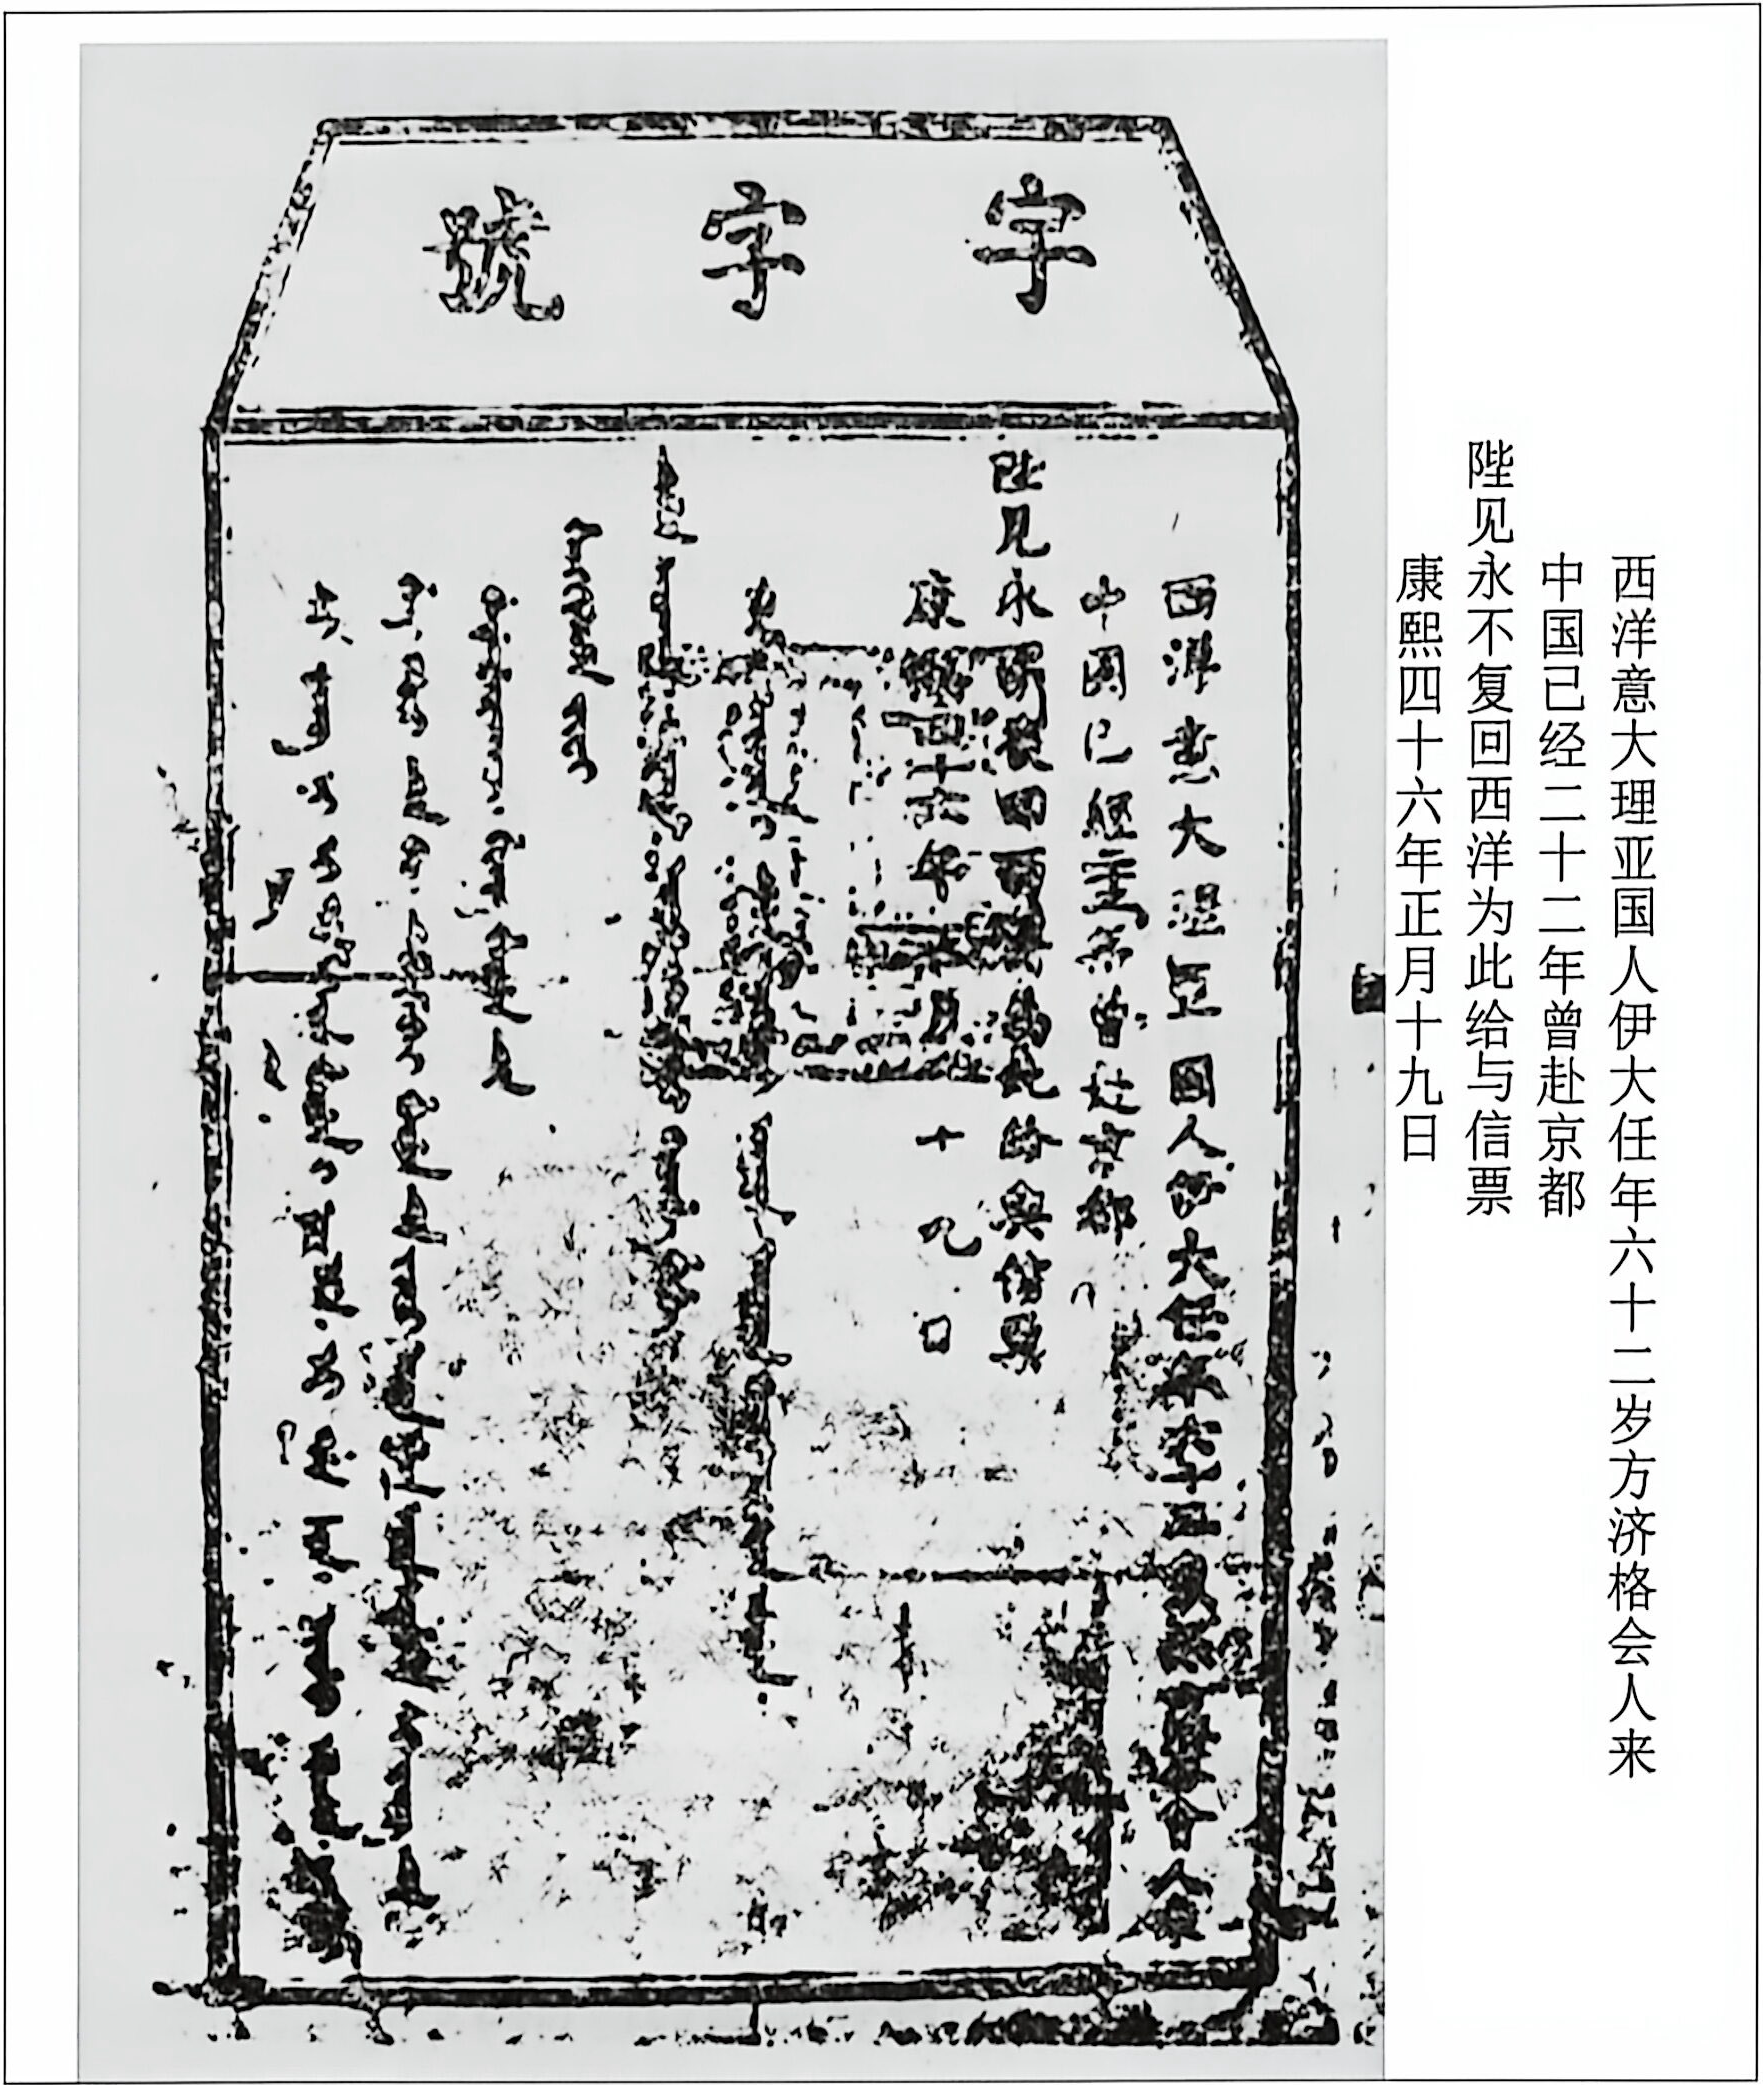
\includegraphics[width=\linewidth,height=.76\textheight,keepaspectratio]{assets/figures/missionary-permit.png}
\caption*{图4.1\quad 内务府发于传教士的印票}
\BookFloatNotes{图片来源：鞠德源，《清宫廷画家郎世宁年谱》，34。}
\end{figure}%
礼部发放的度牒等官文是不一样的。当时在北京的德国传教士纪理%
安（1655—1720）在用拉丁文发回欧洲的记录中还专门对比过：%
\par
% 原书页码：127；段落
{\bookkai 那些说我们与和尚地位差不多的说法是不对的。和尚受官僚机构}%
{\bookkai 以及地方官的管辖。但我们拿的印票，不受制于任何官僚机构。而且}%
{\bookkai 就像赫世亨（康熙身边的包衣奴才）所说的那样，官员们看到我们的}%
{\bookkai 票后都会礼让三分。这些票都是皇上亲自发放的，又称“龙票”，上}%
{\bookkai 面有龙的标志，外加内务府总管的印。这样一来，有这个票的人就不}%
{\bookkai 受普通官员的管辖了。}%
\par
% 原书页码：127；段落
{\bookkai 而且，欧洲人拿到的这个票是在皇帝御前发放的。这在中国来说}%
{\bookkai 是最高的待遇，象征着一种特别的恩宠。当然，这个票也不能拿出去}%
{\bookkai 胡乱使用，小心谨慎也是必不可少的。\NoteRef{4}{32}}%
\par
% 原书页码：127；段落
上面纪理安用拉丁文写给欧洲人看的文字，当然有在父老乡亲面前炫%
耀地位的意思。但了解大清官僚运作机制以后，就知道他说的是真的。%
内务府的人，在地方上确实享有特殊待遇，他们确实不受地方官直接%
管辖。内务府的人如果在地方上犯了事，地方官员要知会内务府，由%
内务府来处理，这种法律上的特权，就是纪理安所谓“不受制于任何%
官僚机构”的意思。而且地方官员都知道传教士是内务府的人，也确%
实对他们礼让三分，或说是敬而远之，因为最让地方官员忌惮的是内%
务府的人有和皇帝的联系渠道。举个例子，在真定府（治所在今河北%
正定县），传教士派去收地租的人和租户因为纠纷打架。注意，只是%
打架，并没有伤亡。这样鸡毛蒜皮的地方事件康熙竟然知道了，还写%
了专门的谕旨给直隶巡抚赵弘燮，谕旨是这样写的：%
\par
% 原书页码：128；段落
{\bookkai 近日闻得京中西洋人说，真定府堂内有票西洋人偶有比此争地，}%
{\bookkai 以致生祸授打等语，未知虚实；但西洋人到中国将三百年，未见不好}%
{\bookkai 处。若事无大关，从宽亦可。尔细查缘由情形，写折奏闻。\NoteRef{4}{33}}%
\par
% 原书页码：128–129；段落（跨页续段）
收到这封谕旨时，赵弘燮根本没听说过这事，地方上没有向他汇报%
过。站在直隶巡抚赵弘燮的角度，他接到谕旨后，会从中看到什么，%
想到什么？第一，康熙专门在西洋人前面加了“有票”二字，也就%
是告诉巡抚，这不是普通西洋人，是拿着康熙印票的西洋人。康熙%
的潜台词是，这些洋人是我府中的人，所以他要过问这件事。第二，%
赵弘燮应该立刻感受到了传教士在京城的能量。一桩地方上的小事，%
他都还不知道，传教士已经让皇帝知道了。第三，他不知道传教士%
在康熙那里是怎么报告这件事的，也不知道康熙迫问这件事的目的%
何在。赵弘燮看完谕旨后应该是有很多想法和顾虑的，这也在他后%
来的汇报中体现了出来。这样一桩小案子他啰啰唆唆地写了很长的%
报告，生怕漏掉了任何细节。从报告来看，事件其实很简单，一个%
当地人把土地典当给了传教士，然后他继续在土地上耕作，这样相%
当于他是土地上的佃户，应该交租。但他拖欠了地租，传教士于是%
派仆人去催缴。在催缴过程中两边从争吵逐渐变成了互相厮打，但%
双方似乎都未有受伤。所以就案情来看，这是一桩再普通不过的地%
方打架斗殴事件。了解全部案情经过后，大概赵弘燮也觉得自己有%
点冤，还专门在报告最后注明这个案子只是地方上的斗殴事件，当%
地已经处理过了，按朝廷规定，这种小案件是不上报朝廷的。这也%
是在向康熙解释，为什么他不知道这个案子，也没有上报过。这个%
% 原书页码：129；图表（图题／表题所在页）
\begin{figure}[tbp]\phantomsection\label{fig-148-0}
\centering
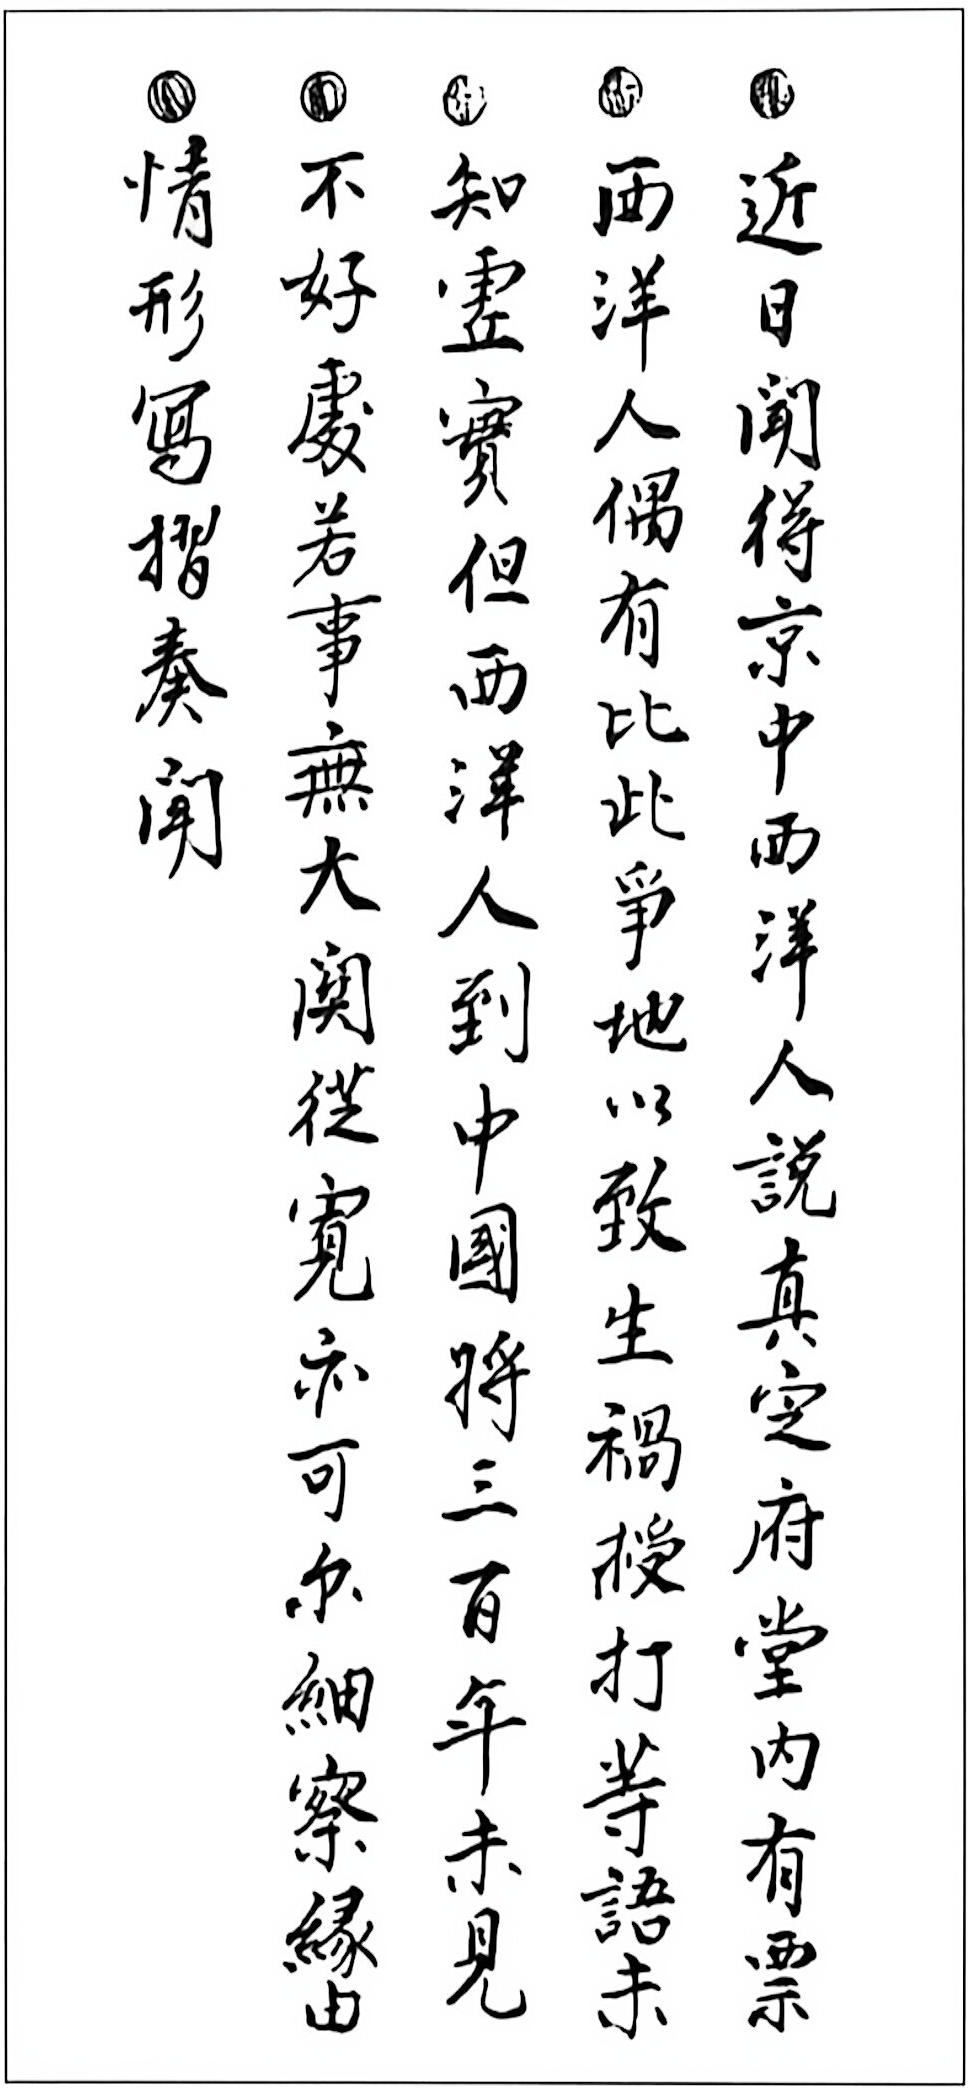
\includegraphics[width=\linewidth,height=.76\textheight,keepaspectratio]{assets/figures/kangxi-fighting-edict.png}
\caption*{图4.2\quad 康熙过问西洋人打架案谕旨}
\BookFloatNotes{图片来源：《康熙朝汉文朱批奏折汇编》，6：108。}
\end{figure}%
案件一来一往似乎只是康熙%
和赵弘燮在对话，但可以想%
象赵弘燮接到康熙谕旨以%
后，一路追查到地方，涉及%
的每一个官员都会很惊讶，%
为什么皇帝会来追查过问这%
种小案子，当然也会马上明%
白这些内务府名下传教士的%
能量。同时，报告中能看出%
赵弘燮也完全领会了康熙谕%
旨中偏袒传教士的意思，因%
为康熙在谕旨中已经明写%
了，尽管他“未知虚实”，%
还是评点了一句“但西洋人%
到中国将三百年，未见不好%
处”。这个“但”字相当于%
已经给案子定调了。身为直%
隶巡抚的赵弘燮不可能看不%
出这个“但”字的意思。所%
以报告最后的结论是康熙圣明，西洋人确实没有什么错。%
\par
% 原书页码：129–130；段落（跨页续段）
其实还没有发票给传教士的时候，康熙就在全国范围内关照传教%
士的生活了。比如1690年，康熙用满文发过私信给山东巡抚，说他%
听说山东有人诬告传教士。山东巡抚接到康熙私信当天，就赶紧派%
人跑遍了省城四处打听，随即上奏康熙，说他打听了一圈，没听说%
有告西洋人的事情。过了四天以后，他终于打听到了，在东昌府茌%
平县（今属山东聊城）下，一位地方居民把房屋卖给了传教士，买%
卖结束后，卖家的一个兄弟出现了，不同意买卖，因而诬告了西洋%
人。案子很小，但康熙这样亲自派人传信过问，着实把山东巡抚吓%
着了。当时通信手段有限，山东巡抚夜以继日加班加点才终于在四%
天之内把案件搞明白。所幸案情简单，涉案问题单一，没惹出大麻烦。%
给康熙的密折中说完案情后，山东巡抚赶紧称赞：“西洋人学问真实，%
断不为不义之事，臣亦知之。”最后，他向康熙认错，说这样的事发%
生了一个多月他都不知道，是他的失职。\NoteRef{4}{34}%
\par
% 原书页码：130–131；段落（跨页续段）
在生活中，康熙对待传教士也确实像一个满人大家族中的主子一%
样，内务府就相当于传教士在中国的娘家。他们想修教堂的时候，会%
写申请到内务府要求拨给土地。\NoteRef{4}{35}传教士需要钱来维修教堂的时候，%
是康熙从他自己的小金库中拿钱出来私下借给他们。\NoteRef{4}{36}他们生病了，%
内科病康熙给他们找中医，骑马摔伤则给他们找满人或者蒙古人医生。%
春节时，康熙按照他打赏自己周围包衣奴才的惯例打赏传教士。传教%
士认为刑部处理与他们相关的案子有不公，康熙就找内务府出面帮他%
们和刑部打招呼。\NoteRef{4}{37}传教士需要马匹出远门，又是内务府给他们开条%
子到兵部去借马（类似于现在使用公家车辆）。\NoteRef{4}{38}传教士修教堂，需要%
木头，内务府又发信给工部，让工部把库存的杉木借给传教士。\NoteRef{4}{39}在%
康熙决定委派耶稣会白晋神父作为他的特使出使欧洲后，教皇使节对%
白晋的身份是否适合出任康熙特使表示了疑问，康熙就直接说白晋是%
他“御前之人”而且是“府中之人”。\NoteRef{4}{40}当康熙得知教皇使节和耶稣会%
神父私下争执时，说了他为什么始终无条件支持耶稣会神父，康熙的%
话很直白：%
\par
% 原书页码：131；段落
{\bookkai 我们就是养一条小狗，也不允许别人欺负。更何况是这些我小时}%
{\bookkai 候就在我周围，跟了我四十五年，我信任的人。\NoteRef{4}{41}}%
\par
% 原书页码：131；段落
这些“人”指的就是北京的耶稣会士。当康熙用“小狗”作比喻，说明%
打狗欺主道理的时候，就是在讲最传统的满人游牧文化。狗和主人之间%
的关系，恰恰是满人中主奴关系最形象的比喻。康熙在杀索额图时就%
说“养犬尚知主恩”，以此表示索额图不知好歹。白晋在一封用满语写%
给康熙的折子中，也跟着满人习惯叫康熙为主子，称康熙为“明主”“大%
主”和“仁主”（详见第五章）。称康熙为“主”（满语Ejen）就是主奴%
关系下的称谓。在传统中国的文臣奏议中都是称“皇上”或者“圣上”。%
“上”是代表皇帝的字眼。称康熙为“主”的，都是康熙的奴才。比如%
在曹寅的奏折中一般不称“圣上”，而是称“圣主”或者“主上”等。%
而康熙也以主子自称，一次给曹寅儿子的回复中，让他把听到的地方上%
的笑话也向他汇报，说让“老主子笑笑也好”。\NoteRef{4}{42}当然，和曹寅父子一样，%
处于主奴关系中的传教士，也享受着各种主奴关系下的特权。%
% 原书页码：131；标题
\subsection{新来的传教士}
\par
% 原书页码：131–132；段落（跨页续段）
鉴于康熙对传教士的关照，和1692年颁布的容教诏书，法国传教%
士认为当时中国有极好的传教机会。李明和白晋人华几年后又回到欧%
洲，撰文著书介绍中国，宣传中国友好的传教氛围。他们介绍中国的%
书都是当时的畅销书，起到的宣传效果也很明显。1703年，仅法国一%
个国家，就有超过三十位神父出发前往中国。\NoteRef{4}{43}南怀仁在世时就很苦%
恼只有很少的传教士来华。为此，他在1678年发信到欧洲鼓励更多%
传教士来华。而在他发信的十年间，整个欧洲总共只有七位神父来到%
中国。\NoteRef{4}{44}%
\par
% 原书页码：132；段落
1699年，白晋从欧洲出发返回中国，有十一位神父和他一同来到%
中国。白晋是康熙的西学老师，在宫里教过康熙好几年，同时他又是%
康熙派回欧洲招募传教士的，算是康熙的钦差。他离开北京的时候，%
已经和广州各级官员打过交道。回到广州的时候，就有水军官员一眼%
认出他来。他在广州上岸后，第一件事就是直接去找两广总督石琳%
（1689—1702年在任），请石琳转告北京，他已经回来了。同时他还请%
石琳帮忙安排，船上有几个人生病了，需要治疗。石琳当然将一切都%
安排周到。据白晋说广州大小官员都来拜访他，持续了三天。白晋乘%
坐的船是法国国王派的船，船长和手下看到白晋受到的礼遇都惊叹不%
已，觉得不可思议。白晋作为一个法国人，一到广州不仅能获得当地%
最高官员接待，而且大小官员还争相来拜访。当然这一切都是因为白%
晋的特殊身份，当地官员知道尽管他没有官衔，但却是天天跟在皇帝%
身边的人，所以大小官员都争相和白晋往来，大献殷勤。\NoteRef{4}{45}%
\par
% 原书页码：132–133；段落（跨页续段）
康熙知道白晋返回后，从内务府里派了一人到广州迎接，而且让%
官员免除了白晋所乘法国船只的各种税费。当时康熙正好在江南南%
巡，便命白晋带着新来的传教士北上，在康熙的龙船上会面。广州官%
员知道一船人要北上见皇上，又热情地为这些新来的洋人送别。最终%
白晋一行在离扬州不远的地方，上船拜见了康熙。白晋说他见到康熙%
时，康熙在窗边，看到他，便问：“身体可好？”完全是老朋友重逢的%
画面。白晋说，当时官员都在，谈话不能深人，大家也比较拘谨。到%
了晚上，他带着新来的传教士再和康熙相见，谈了很久，而且氛围也%
比较随意。\NoteRef{4}{46}%
\par
% 原书页码：133；段落
在船上见面后，康熙让白晋选出五人留在京城听候差遣。这批传%
教士还见了张诚神父。张诚1688年到京后就得到康熙赏识，后来代表%
清朝与俄罗斯谈判《尼布楚条约》，又立了大功。这之后，他就是最%
常出现在康熙身边的传教士之一。康熙三次出击塞外亲征准噶尔，张%
诚都陪同在侧。后来每次南巡，康熙也把张诚带在身边。新来的传教%
士都清楚，他们在这个遥远的异乡，一来就能得到从上至下的照顾和%
恩惠，都是张诚这样侍候在皇帝身边的传教士的功劳。%
\par
% 原书页码：133–134；段落（跨页续段）
1693年，康熙又把内务府一套院子送给了法国传教士，感谢他们%
治好了他的病。当时康熙得了疟疾外加发烧，朝廷内的中医治不好，病%
情一天一天加重。张诚、洪若翰、刘应三位法国神父毛遂自荐为康熙医%
治。他们用金鸡纳树的树皮治好了康熙的病。\NoteRef{4}{47}金鸡纳树原产南美，当%
地人很早就用它来治疗疟疾和发烧，后来耶稣会神父传教到那里，知%
道了这个树皮的妙用，便把它作为一味神药带到世界各地治疗发烧（这%
个树皮治病的有效成分是奎宁）。康熙送的院子在故宫外西北方向不远%
处，由于位置离故宫很近，在当时就属于一流的地段（见图4.3）。这个%
院子后来成了法国传教士的主要住所。院子的位置也在实际生活中缩%
短了法国传教士人宫觐见康熙的距离。第二年，法国传教士得知院子旁%
的一处空地也是内务府的，而且还知道内务府里的太监正在打这块地%
的主意，他们就在太监提交申请之前向内务府申请了这块地，说希望%
在这里修一处教堂。后来康熙权衡以后，把这块地一分为二，给了传教%
士和太监各一半。传教士没有把自已当外人，还跟内务府的太监争“地%
盘”。不过，传教士是很会搞关系的，他们和内务府中的太监相处融洽，%
并没有因为地皮申请影响到双方的关系。\NoteRef{4}{48}%
% 原书页码：134；标题
\subsection{关系网}
\par
% 原书页码：134；段落
新来的传教士去到各个地方传教前，老传教士都会传授他们各种%
注意事项，中国的习俗，与官员打交道的策略，哪些能干哪些不能%
干，等等。不过，到了地方以后，传教士还是会遇到各种预想不到的%
事，这时候京城的传教士就是给他们解决问题的人。比如传教士利圣%
学（Charles de Broissia）到宁波传教，准备在那里修一座教堂。他到宁%
波后，很快就和当地三位地方官搞好了关系，并得到三位官员默许，%
着手在宁波新修教堂。教堂还在修建过程中，三位官员陆续调任其他%
地方。新来的地方官对修教堂一事不予支持。利圣学想了各种办法巴%
结新来的官员，并告诉他其他地方也在修教堂，该官员坚持要通报礼%
部，让北京来裁定。官员认为之前的容教诏书虽未禁止建造新的教堂，%
但也并没有允许新建。\NoteRef{4}{49}%
\par
% 原书页码：134–136；段落（跨页续段，中间插图不另起段）
在知道事情捅到了礼部后，张诚和在京的传教士都很担心，如果%
礼部做出禁修教堂的决定，那么以后全国各地传教都会受到影响。张%
诚动用了在京城的关系，在礼部部议之前，私下找到了礼部尚书。好%
在礼部尚书对该案没有什么异议，表示会给出满意结果。几天后，礼%
% 原书页码：135；图表（图题／表题所在页）
\begin{figure}[tbp]\phantomsection\label{fig-154-0}
\centering
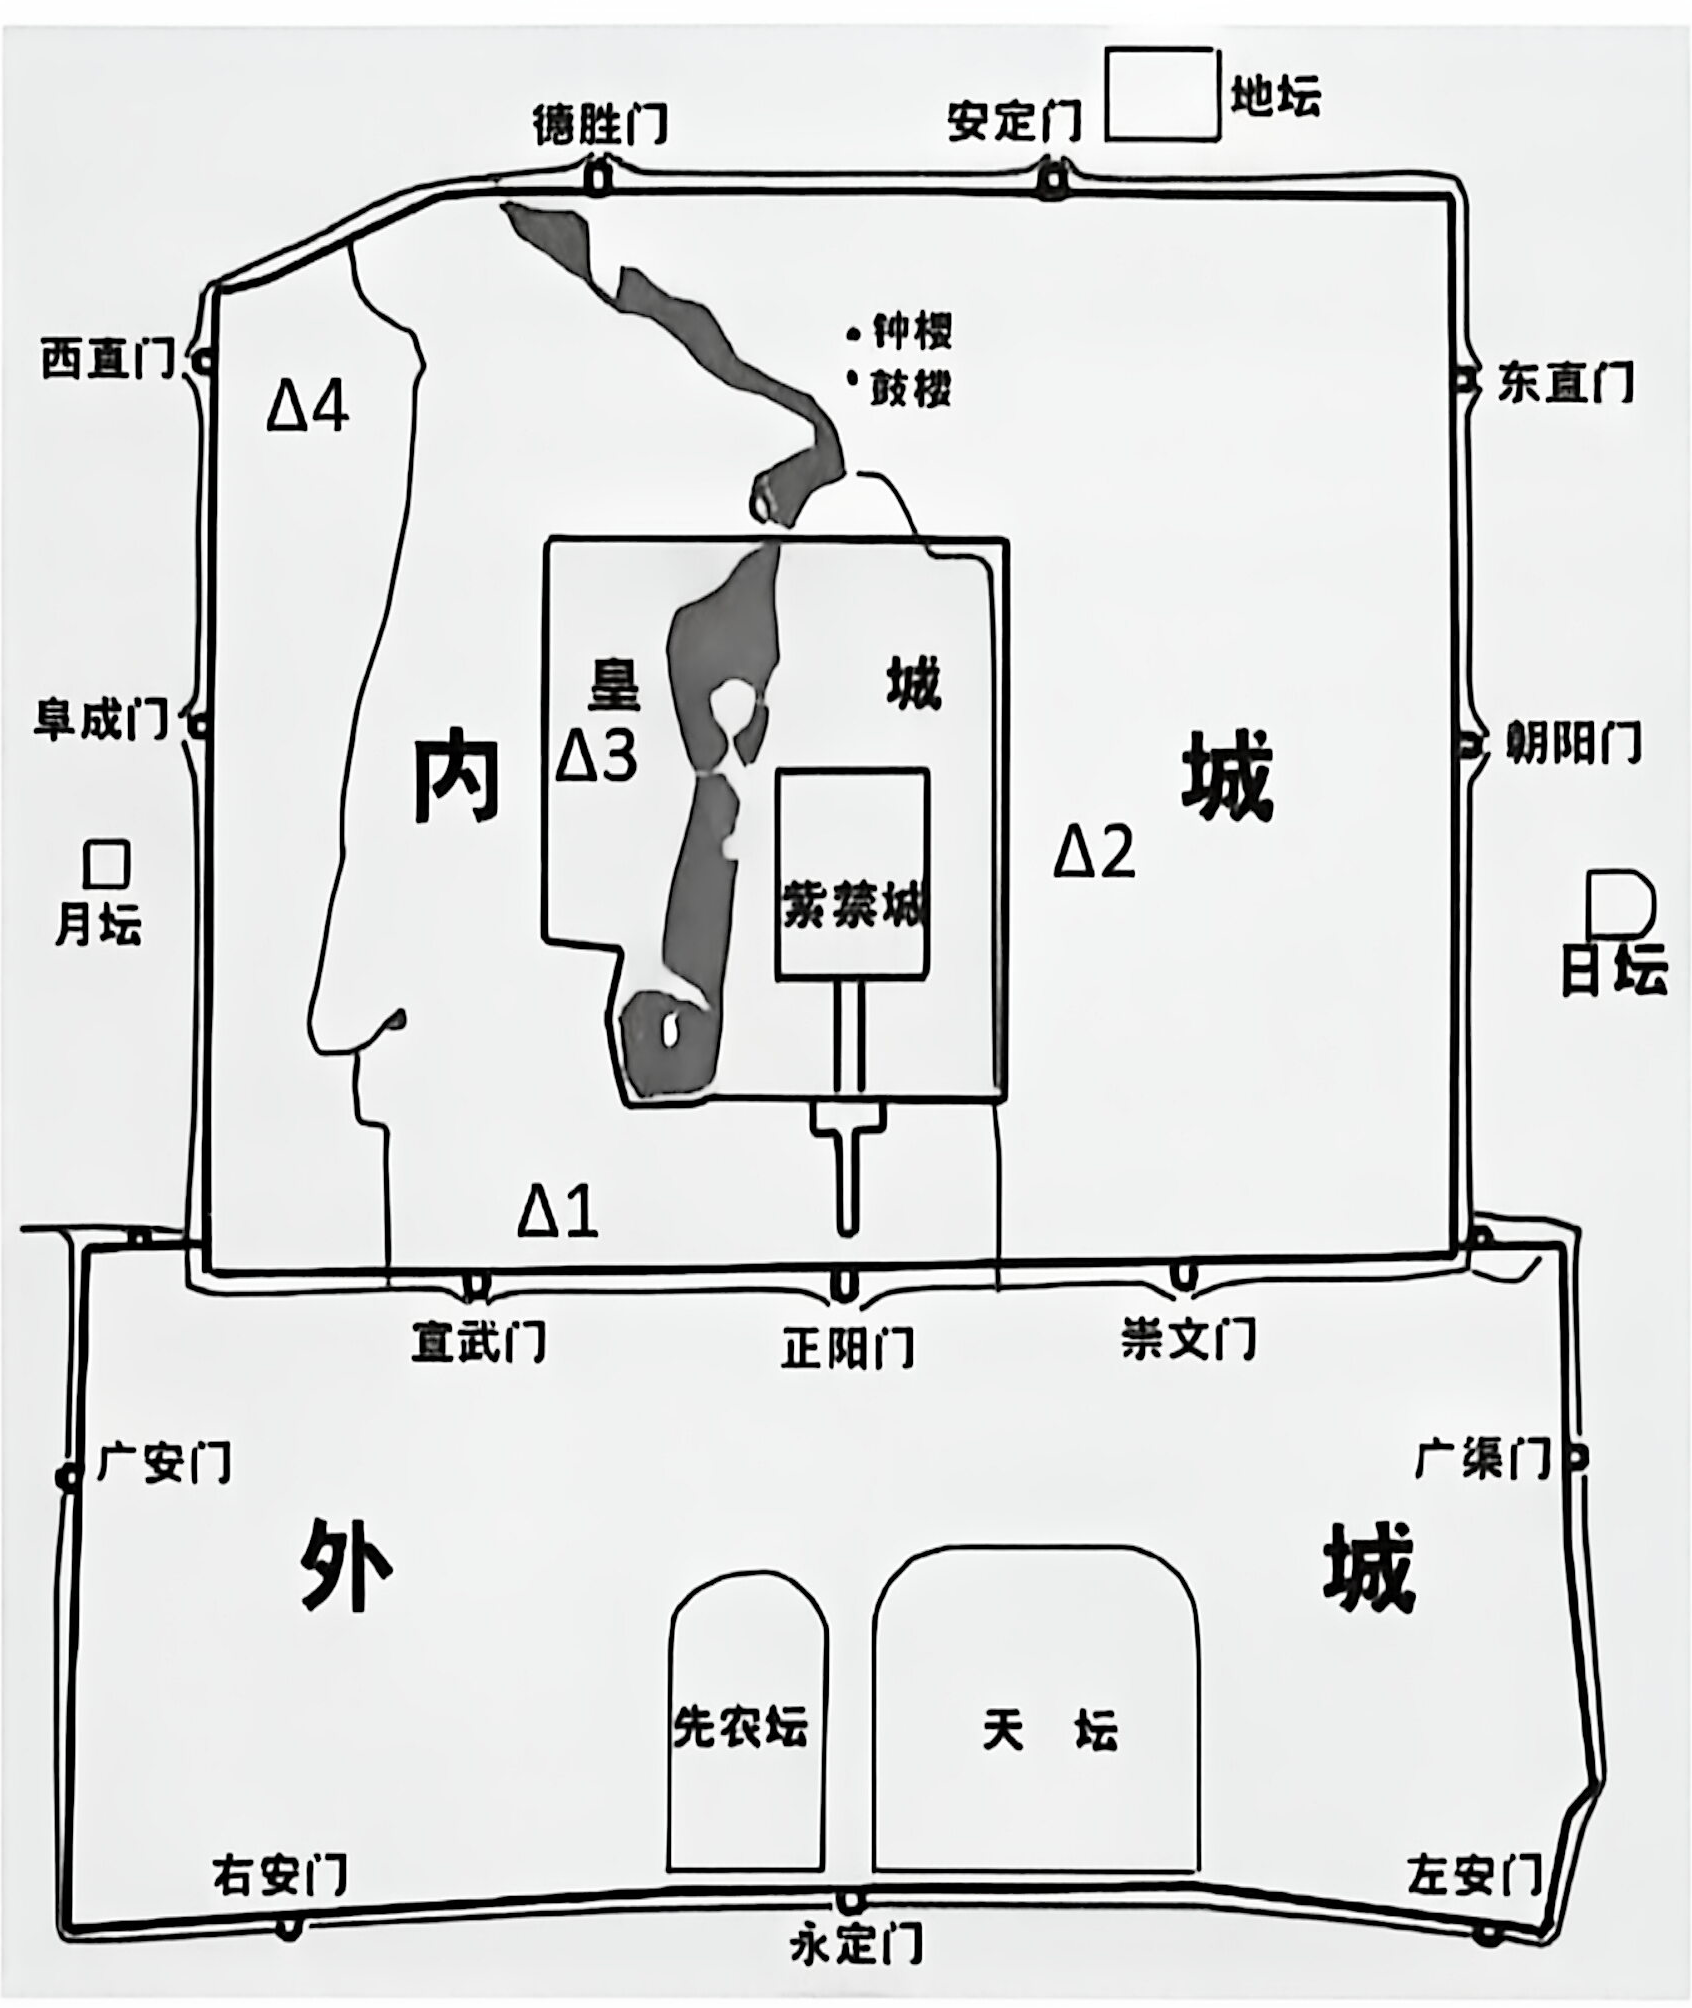
\includegraphics[width=\linewidth,height=.60\textheight,keepaspectratio]{assets/figures/beijing-churches.png}
\caption*{图4.3\quad 清初北京教堂位置图}
\BookFloatNotes{△1：南堂，1605年利玛窦始建，1650年汤若望翻新。又称宣武门天主堂。\par\noindent △2：东堂，1655年利类思和安文思创建。又称圣若瑟堂。\par\noindent △3：北堂，1703年法国传教士创建。又称西什库天主堂。\par\noindent △4：西堂，1723年（雍正元年）德里格创建。又称西直门天主堂。}
\end{figure}%
部给出了允许修建的结论。理由是既然当地能允许修寺庙，那么修教%
堂也应该允许。\NoteRef{4}{50}潜台词是让地方官把教堂当成寺庙一视同仁处理。%
尽管这件事情最后有了满意的结果，京城的传教士还是感觉压力很大，%
通知各地传教士，尽量把地方上的问题就地解决，不要把事情闹到京%
城来。他们认为不可能每一次都有好运气，如果礼部哪次因为某个地%
方案件给出一个不利的结果，那么这个结果会在全国范围都产生负面%
影响。%
\par
% 原书页码：136；段落
由于有这个就地解决问题的方针，洪若翰神父在湖北黄州修教堂%
的计划就只好暂停了。按洪若翰记载，黄州的地方官不仅不同意修教%
堂，还默许道士和地痞在他准备修教堂的地方闹事。洪若翰说他走了%
二百多里去找湖北巡抚。尽管巡抚彬彬有礼地接待了他，但洪若翰%
明显感觉到巡抚在刻意和他保持距离，因为连他带去的小礼品，巡%
抚都不接受。巡抚给出的意见很像托词，说地方要修教堂的话，他%
必须上报礼部。要是北京同意修，他也没有意见。洪若翰在巡抚那里%
无功而返，只好把问题反映给了张诚。张诚通过他京城的关系网，竟%
然找到了巡抚在京城国子监当差的大儿子。传教士并没有详述他们是%
如何打通关节找到这个人的，只是说巡抚大儿子一封家书回去，一切%
都解决了。巡抚收到家书以后，很快找到了当地的耶稣会神父樊西元%
（Jean-Simon Bayard）。传教士的记录中说，巡抚和樊西元聊天中并没有%
谈到修教堂的事，只是谈了谈传教士学习中文等无关的事。不过会谈%
结束后，巡抚就给黄州地方官去了信，信中还附上了康熙的容教诏令。%
地方官接到信后，态度大变，亲自带着礼物找到洪若翰，并在传教士%
住处周围张贴告示，表示允许修建教堂。\NoteRef{4}{51}%
\par
% 原书页码：136–137；段落（跨页续段）
尽管这些传教士是外国人，但在1700年代，他们对中国人情社会%
下各种关系的运作是很老练的。特别需要注意的是，上面两个例子都%
是张诚自己一手搞定的，并没有求助于康熙。比起南怀仁，张诚可以%
说在北京官场已经青出于蓝而胜于蓝了。回想1673年，把一个传教%
士从浙江转去西安这样的芝麻小事，南怀仁都拿不到礼部的批文，还%
需要康熙介人。而此时的张诚已经可以直接私下去找礼部尚书交流了，%
这说明传教士在京城权力圈中已建立了自己的关系网。不过，话又说%
回来，跟权贵交往过密也是双刃剑，遇到政治风波，难免被牵连。后%
来天主教在雍正初年被禁，就和传教士与京城各方权贵交往过密有关。%
这是后话了。%
% 原书页码：137；标题
\subsection{介绍中国}
\par
% 原书页码：137–138；段落（跨页续段）
传教士在朝中有人，同时又有内务府关照，这是地方官都知道%
的。这为传教士在各地的活动提供了方便。当时传教士以及欧洲商%
人走遍了世界各地以后，都认为中华文明是地球上唯一可以和欧洲%
文明媲美的。传教士到中国来传教的同时，带来了西方的科学知识，%
但同时他们也在全方位地学习、考察中国的方方面面。来华的很多%
传教士，自身就是一流的学者。汤若望和南怀仁都是科学素养极高%
的全能型传教士。后来来华的传教士中更是有很多精英。特别是法%
国派来的传教士，这和法国国王路易十四的重视有关。比如第一批%
来华的五位耶稣会传教士白晋、张诚、洪若翰、李明和刘应。其中%
的洪若翰神父，他在法国就是与法国科学院院士一起做研究的。在%
入华航行路上，他就在观测星空，船航行到赤道，他记录下了南半%
球能看到的星空。从他的记录中可以看出，他知道哪些信息有价值，%
哪些是欧洲科学观察急需验证的部分。张诚在欧洲是神父，同时还%
在大学里面教数学。这五位神父在出发之前，法国科学院还给他们%
专门开了各种科学讲座，让他们在数学、天文学、地理学、植物学、%
动物学等众多学科中都有一定的知识储备。\NoteRef{4}{52}这样到中国，如果遇到%
相关发现，才有能力做记录。%
\par
% 原书页码：138；段落
白晋神父其实在数学、天文、技术等方面都是行家，但是他到%
中国后迅速被浩瀚的中国古代典籍吸引。人华后，从一字不识开始%
学习汉语，到博览中国古书，最后深陷在《易经》研究中不能自拔。%
康熙对此还发过脾气，认为白晋不务正业，耽误了他给安排的工作。%
康熙在平定三藩和准噶尔以后，开始丈量国土，绘制全国地图。这%
种工程自然是传教士主导，但这个项目太大，需要大量人手。长城%
外的区域，测量绘制地图，不免风餐露宿，是件苦差事。康熙知道%
白晋当时忙着研究《易经》，但无奈人手不够，还是派他去测绘长城%
部分。结果出去没多久，康熙身边的包衣奴才就报告说，白晋坠马%
摔伤了，在回京的路上。康熙听完很生气，马上意识到这是白晋在%
找借口返回京城。康熙还察觉到，打报告的包衣奴才在帮白晋打圆%
场，便反问道，要真是坠马，就该在坠马的地方养伤，养好了继续%
勘测。这坠马后就回京是什么意思？\NoteRef{4}{53}%
\par
% 原书页码：138–139；段落（跨页续段）
被《易经》吸引的还有法国耶稣会傅圣泽神父。傅圣泽神父是%
1699年人华的，他最初在福建、江西一带传教。傅圣泽深爱中国古代%
经典，其中最让他痴迷的是老子的《道德经》和儒家六经之一的《易%
经》。他钻研《易经》的角度很独特，认为《易经》中的卦象和《圣%
经·旧约》中的一些图像是相通的。他的学问大，在中国传教士内部%
都是公认的。后来有传教士向康熙推荐傅圣泽，康熙便把他召到了北%
京。但傅圣泽对出入宫廷没有兴趣，大约认为这会影响他的研究。他%
几次给康熙的回复都是他水平有限，有很多不懂。但实际他到北京后，%
一直专心研究中国古代典籍，同时忙着在当时北京琉璃厂附近的旧书%
市场淘中国古书。他在中国待了二十年。在1720年返回欧洲时，他购%
买了一千余册中国经典运回欧洲去。回欧洲后不久，便被教皇任命为%
主教。傅圣泽本来就是富家子弟出身，去中国前他在哲学、神学和数%
学方面的造诣已经在法国有名气了。现在他又到中国学了二十年的中%
国经典，又把这些经典带回欧洲翻译，对当时的欧洲学者来说，大约%
相当于我们理解中“唐僧取得真经归来”的感觉。法国当时的大师如%
伏尔泰和卢梭都数次找到傅圣泽当面请教中国方面的问题，以及他对%
很多哲学问题的见解。傅圣泽把中国古代主要的经典都带回了法国，%
开启了法国的汉学研究进程，以至于后来两百年，法国在汉学研究领%
域都是欧洲的翘楚。%
\par
% 原书页码：139–140；段落（跨页续段）
当时中国在世界上最著名的物品无疑是瓷器。在江西传教的法%
国传教士殷弘绪（François Xavier d'Entrecolles，1664—1741）详细记%
录了景德镇烧瓷工艺，1712和1720年他写了两份报告发回欧洲。除%
了自己的观察外，他还从当地人那里得到许多烧制瓷器的关键步骤%
信息。他的报告发回欧洲后，很快被翻译成各种欧洲语言。英国和%
德国当时新建的陶瓷作坊，都得益于殷弘绪神父的报告。当时景德%
镇的师傅对景德镇工艺很有信心，不担心技术外传，他们跟殷弘绪%
神父讲，就是景德镇的熟练工人，换到福建去烧瓷，烧出来的成品%
都要差一截。当时的解释是，景德镇陶瓷的核心是当地的土。这个%
原材料其他地方没有。殷弘绪还介绍说，由于火候控制的原因，整%
窑瓷器全部报废的事经常发生。他说每一个发财的老板背后，都有%
“百名破产者”。这也跟欧洲人解释了为什么中国产的瓷器会那么贵，%
是当时的奢侈品。\NoteRef{4}{54}殷弘绪神父在报告中还特别惊叹于景德镇的治%
安，称当地有三千座瓷窑，人口稠密，而且每天往来商船不断，但%
神奇的是当地只有一位朝廷官员。治安靠商户选出来的地保负责照%
看。作为一个走过世界很多地方的欧洲人，他称景德镇的“治安制%
度很令人钦佩”\NoteRef{4}{55}。殷弘绪神父当时能在饶州和景德镇往来自由，得益%
于各级官府的保护。他在当地的教堂经常还会有官员来拜访。景德%
镇由于进出口瓷器，洋人的商船常到江西来。康熙1708年废太子后，%
经常心慌心悸，在北京传教士介绍下，他喝了少量西洋葡萄酒后症%
状有所改善。为此他晓谕江西巡抚，在来往西洋人那里收集葡萄酒。%
而在饶州（景德镇是当时饶州府下面的一个镇）传教的殷弘绪自然%
也就得到江西巡抚的特别关照。%
\par
% 原书页码：140–141；段落（跨页续段）
康熙在传教士的推荐下使用了一些西医的疗法，同时康熙也派中%
医大夫给传教士治病。传教士在中国见识过中医的疗效，包括针灸。%
传教士到世界各地传教，医疗都是他们的强项，也就是说他们可以通%
过治病来接触和感化信徒。但中国是个例外，尽管西医在某些病的治%
疗上有特色，但是对于大部分的病他们承认是不如中医的。这也是为%
什么传教士是用天文历算而不是医学来进入中国的原因。人都有生老%
病死，传教士也不例外。从第一批传教士明代人华开始，他们很快就%
发现中医在很多病的防治上都有独特思路和疗效。最早系统介绍中医%
和中药的传教士是邓玉函（Johann Schreck，1576—1630）。邓玉函万%
历年间人华，是明清时期所有来华传教士中在欧洲科学界地位最高的%
一位。他年轻时是现代代数创始人韦达的助手，后来是伽利略的学生。%
他早年游学欧洲，在欧洲科学界有一流的关系网。后来他要加入教会，%
伽利略很生气，跟他断绝了往来。到中国后，他被安排去做天文测%
算。当时中国教会需要准确预测日食来显示西方科技的发达，邓玉函%
就发信回欧洲询问天文测算问题。而为他答疑的，是大名鼎鼎的开普%
勒。后来传教士能够很精确地进行日食预测，用的就是开普勒的方法。%
邓玉函在欧洲的本业是植物学和医学。到了中国，遇上中医和中药，%
可以说为他打开了一个崭新的世界。不过可惜的是，在人华十年后%
（1630年），他在一次中药实验中，不幸中毒身亡了。他对中药、把脉、%
针灸都有研究。来华的传教士都希望破解中医治病的原理，他们认为%
中医最神奇的是发现人的脉搏和身体内部运作的关联。古希腊-罗马%
时期西方医学第二号传奇人物盖伦（Aelius Galenus，约 129—216。一%
号人物是现代西医入行誓言的作者希波克拉底）就通过把脉诊病，开%
创了西方的脉学。追随南明朝廷的波兰传教士卜弥格认识到中国的脉%
诊是三维的，医生把脉有按压，以此来感觉脉搏的轻重强弱快慢。他%
把明代成书的《图注脉诀辨真》（一部图文结合便于学习晋代王叔和%
《脉经》的书）翻译成了拉丁文，后来一位荷兰医生把他的翻译收入到%
一本医学方面的综合书籍里。\NoteRef{4}{56}这本书在欧洲多个国家引起了科学家%
的注意。后来的传教士也一直在添补脉学相关的内容。追随南明朝廷%
后来又被孔有德招降的谢务禄神父、第一批来华法国传教士中的李明%
以及1655年荷兰的人华使团，都对脉学有过进一步观察和报告。\NoteRef{4}{57}后%
来西方哮喘研究的奠基人约翰·弗洛耶（John Floyer）就在中国《脉经》%
的基础上，写了一部脉学研究著作。%
\par
% 原书页码：142；段落
传教士走遍世界各地，发现当地的特产，就会介绍回欧洲。比如%
前文说到，传教士在南美看到当地人用金鸡纳树皮治疗疟疾和发烧，%
就把这个树皮传回了欧洲，同时也带到了中国。1693年他们就是用%
金鸡纳树皮治好了康熙。\NoteRef{4}{58}传教士还把巧克力饮料从南美带回欧洲，%
后来也带给了康熙，康熙还很喜欢。\NoteRef{4}{59}他们到了中国，当然也会把中%
国的特产介绍回欧洲。中医在使用自然界动植物上，当时是遥遥领先%
于世界的。这就注定了当时传教士在植物、动物方面有写不完的内容。%
明代早期传教士就写过很多书介绍中国的动植物及其使用方法。殷弘%
绪神父就感叹中医对各种植物的研究太深人了，他根本没有时间完全%
翻阅，只能挑一些欧洲常见的植物看看，然后介绍回欧洲。\NoteRef{4}{60}%
\par
% 原书页码：142；段落
康熙年间的传教士凭借内务府的关系，获知并向西方介绍了一%
些名贵的中药。比如现在价格很贵的虫草。法国传教士巴多明记录说%
虫草贵得不可思议，要四两银子才能买一两。而当时朝廷钦天监监正%
一年的俸禄是一百两银子。也就是说一个朝廷大员的年俸也只能买%
二十五两虫草（跟当下作比，2023年的虫草均价为15万—20万元/%
公斤）。可见虫草清初就很贵。巴多明神父说他没有见过虫草的生长%
环境，只知道它生长在川藏地区。他讲到虫草和人参都有滋补的功能，%
区别是人参有些人服用会引起出血。这和现代讲的人参药性强，虫草%
温补的特性是一致的。而且巴多明神父称他能得到虫草，是因为他和%
川陕总督（他没有明写是谁，可能是岳钟琪）有私交。川陕总督进京%
给皇上带了很多虫草，也送了一些给他。巴多明说他当时正好身体虚%
弱，食用虫草后有显著疗效。当时别人给他介绍的食补方法是用虫草%
炖鸭子。\NoteRef{4}{61}这道食补方子今天依然很流行。%
\par
% 原书页码：143；段落
巴多明还讲到了当时欧洲大量从中国进口大黄。大黄是泻药，可%
以治便秘，这点当时欧洲也发现了。巴多明认为欧洲生服大黄的方法%
比较原始，在治病的同时会引起疼痛。巴多明仔细学习记录了中国炮%
制大黄的过程，再介绍给欧洲。经过中国方式加工后的大黄，再加上%
蜂蜜，巴多明说使用效果好，而且还没有副作用。\NoteRef{4}{62}%
\par
% 原书页码：143；段落
巴多明还提到了阿胶，他不仅知道阿胶是用驴皮制作的，还知道%
制作上等阿胶的阿井。按巴多明的解释，阿井里面的水，和一般的水%
确实有区别，这并不是迷信。北宋《梦溪笔谈》以及明代《本草纲目》%
里面也特别提到过制作阿胶的井里的水有特别之处。巴多明说，那口%
井很珍贵，平时官府在井上贴有封条。巴多明同时提到由于上等阿胶%
产量有限，当时全国各地到处都在卖假阿胶。他说他不能确定阿胶是%
否真有很多疗效，但他可以确认阿胶确实在治疗肺病上有疗效，因为%
有几位传教士都亲身验证过。巴多明也是因为宫里的关系，才能接触%
到上等正宗阿胶。他吃过、用过、研究过，说自已闻一闻就能鉴别出%
阿胶的真假。\NoteRef{4}{63}%
\par
% 原书页码：143；段落
巴多明有很高的语言天赋，他1698年人华后，很快就学会了满%
汉双语的听说读写，而且都很地道。他很快就成为经常在康熙身边的%
传教士，并且和朝廷众多官员都有交往。包括雍正朝的宠臣皇十三子、%
年羹尧和隆科多。他历经康熙、雍正和乾隆三朝，一直混迹在北京的%
权贵圈里。后面章节中还有他的故事。%
\par
% 原书页码：143–144；段落（跨页续段）
像巴多明、殷弘绪这样介绍中国方方面面给欧洲的传教士还有很%
多。康熙年间，有上百个传教士来到中国。每一个入华的传教士在欧%
洲都有他的故乡和他入华前所属的教区，那些地方的教友一直在经济%
上、物质上和精神上支持这些传教士，因而这些传教士也有责任向他%
们在欧洲的故人汇报他们在中国的所见所得。这也是为什么有大量%
传教士介绍中国的文字保留在欧洲的原因。同时入华传教士的学养很%
高，他们很注重宗教以外知识的学习，这样他们在很多领域都有观察，%
写出来的东西也很有价值。北京在康熙年间有三座天主教教堂，这是%
入华传教士的中心。这三座教堂都有专门的图书室，有专门空间存放%
教外图书。那里还存放着欧洲寄过来的书，包括当时欧洲的科学发现，%
同时还有在北京购买的汉文书和满文书。在康熙末年，有朝鲜使团参%
观过北京的教堂，他们声称教堂里藏书超过万册。\NoteRef{4}{64}%
% 原书页码：144；标题
\subsection{中西双向交流}
\par
% 原书页码：144；段落
康熙朝的传教士并不知道百年后欧洲在科学技术方面会有大的突%
破。当时在他们眼中，中国在很多方面都是领先的。所以当时的中西%
交流完全是双向的。欧洲没有而中国有的，他们发现有价值，就传回%
欧洲。比如前文讲到的瓷器烧制技术。同时，欧洲有而中国没有的，%
传教士根据他们传教的需要，就传到中国。比如传教士把欧洲的玻璃%
烧制技术传到了中国。欧洲量产的玻璃在明末传入中国时，中国人最%
初以为是宝石，价格高得离奇。后来法国传教士不仅给中国带来了技%
术，还带来几位欧洲工匠，帮康熙在北京建起了玻璃厂。\NoteRef{4}{65}康熙从南%
方招来学徒，很快北京出产的玻璃制品就可以媲美欧洲，1720年康熙%
赠送给彼得大帝的国礼中就有北京产的玻璃制品。当时的技术传播交%
流是双向的，互通有无。%
\par
% 原书页码：145；段落
当时人的思想中有中外之别，但没有很强的中西之分。特别是对%
实用的东西，有的更多的是有用与没用的区别。就拿中西都有的医学%
来说，康熙和传教士看待医学只有有效与无效的区分或者说适合与不%
适合的区分，并没有现代人有的中西医区分。康熙见识过西药有效后，%
便引进了西药和西医，在他宫里常年储备着多种有用的西药。这些储%
备并不能说明康熙特别看重西医，只是说明他务实。历史中喜欢谈论%
康熙当年被传教士治好了中医都治不好的病，这其实和记录有关，因%
为张诚等法国传教士详细记录了他们治好康熙病的故事。但张诚常年%
被失眠困扰，最后被中医治好了，他就一笔带过。当然也没有哪个中%
医大夫会得意地记录下自己治好失眠的医案。后来的人读到当时中西%
医交流的高光时刻，好像就是西医治好了中医治不了的病，让康熙很%
惊讶。康熙自己和周围的人被中医治好的情况有很多，只是当时人对%
此习以为常，并没有觉得这些是值得记录的事。细读康熙和传教士的%
交往历史就会发现，康熙多次安排医生为传教士治病，可以说每一个%
传教士都接受过中医治疗。%
\par
% 原书页码：145；段落
来华传教士众多，在很多问题上难免观点不同。但就中医和中药%
来说，传教士是一致的赞美惊叹，都是怀着敬意把中医中药介绍回西%
方。欧洲来的人，能在中国找到好的中医看病，都是很高兴的。教皇%
使节来华，路上肠胃出了毛病，进京都是抬入京城的，后来觐见康熙%
时，坐一会儿就很累，身体虚弱，随团的西医一点儿办法都没有。后%
来教皇使节请求康熙的医生给他看病，康熙的中医给他开了一个以槟%
榔为主的方子，把他的肠胃病治好了（方子见图4.4）。%
\par
% 原书页码：145–147；段落（跨页续段）
最后离京的时候，教皇使节已经完全康复，他多次上书康熙表%
% 原书页码：146；图表（图题／表题所在页）
\begin{figure}[tbp]\phantomsection\label{fig-165-0}
\centering
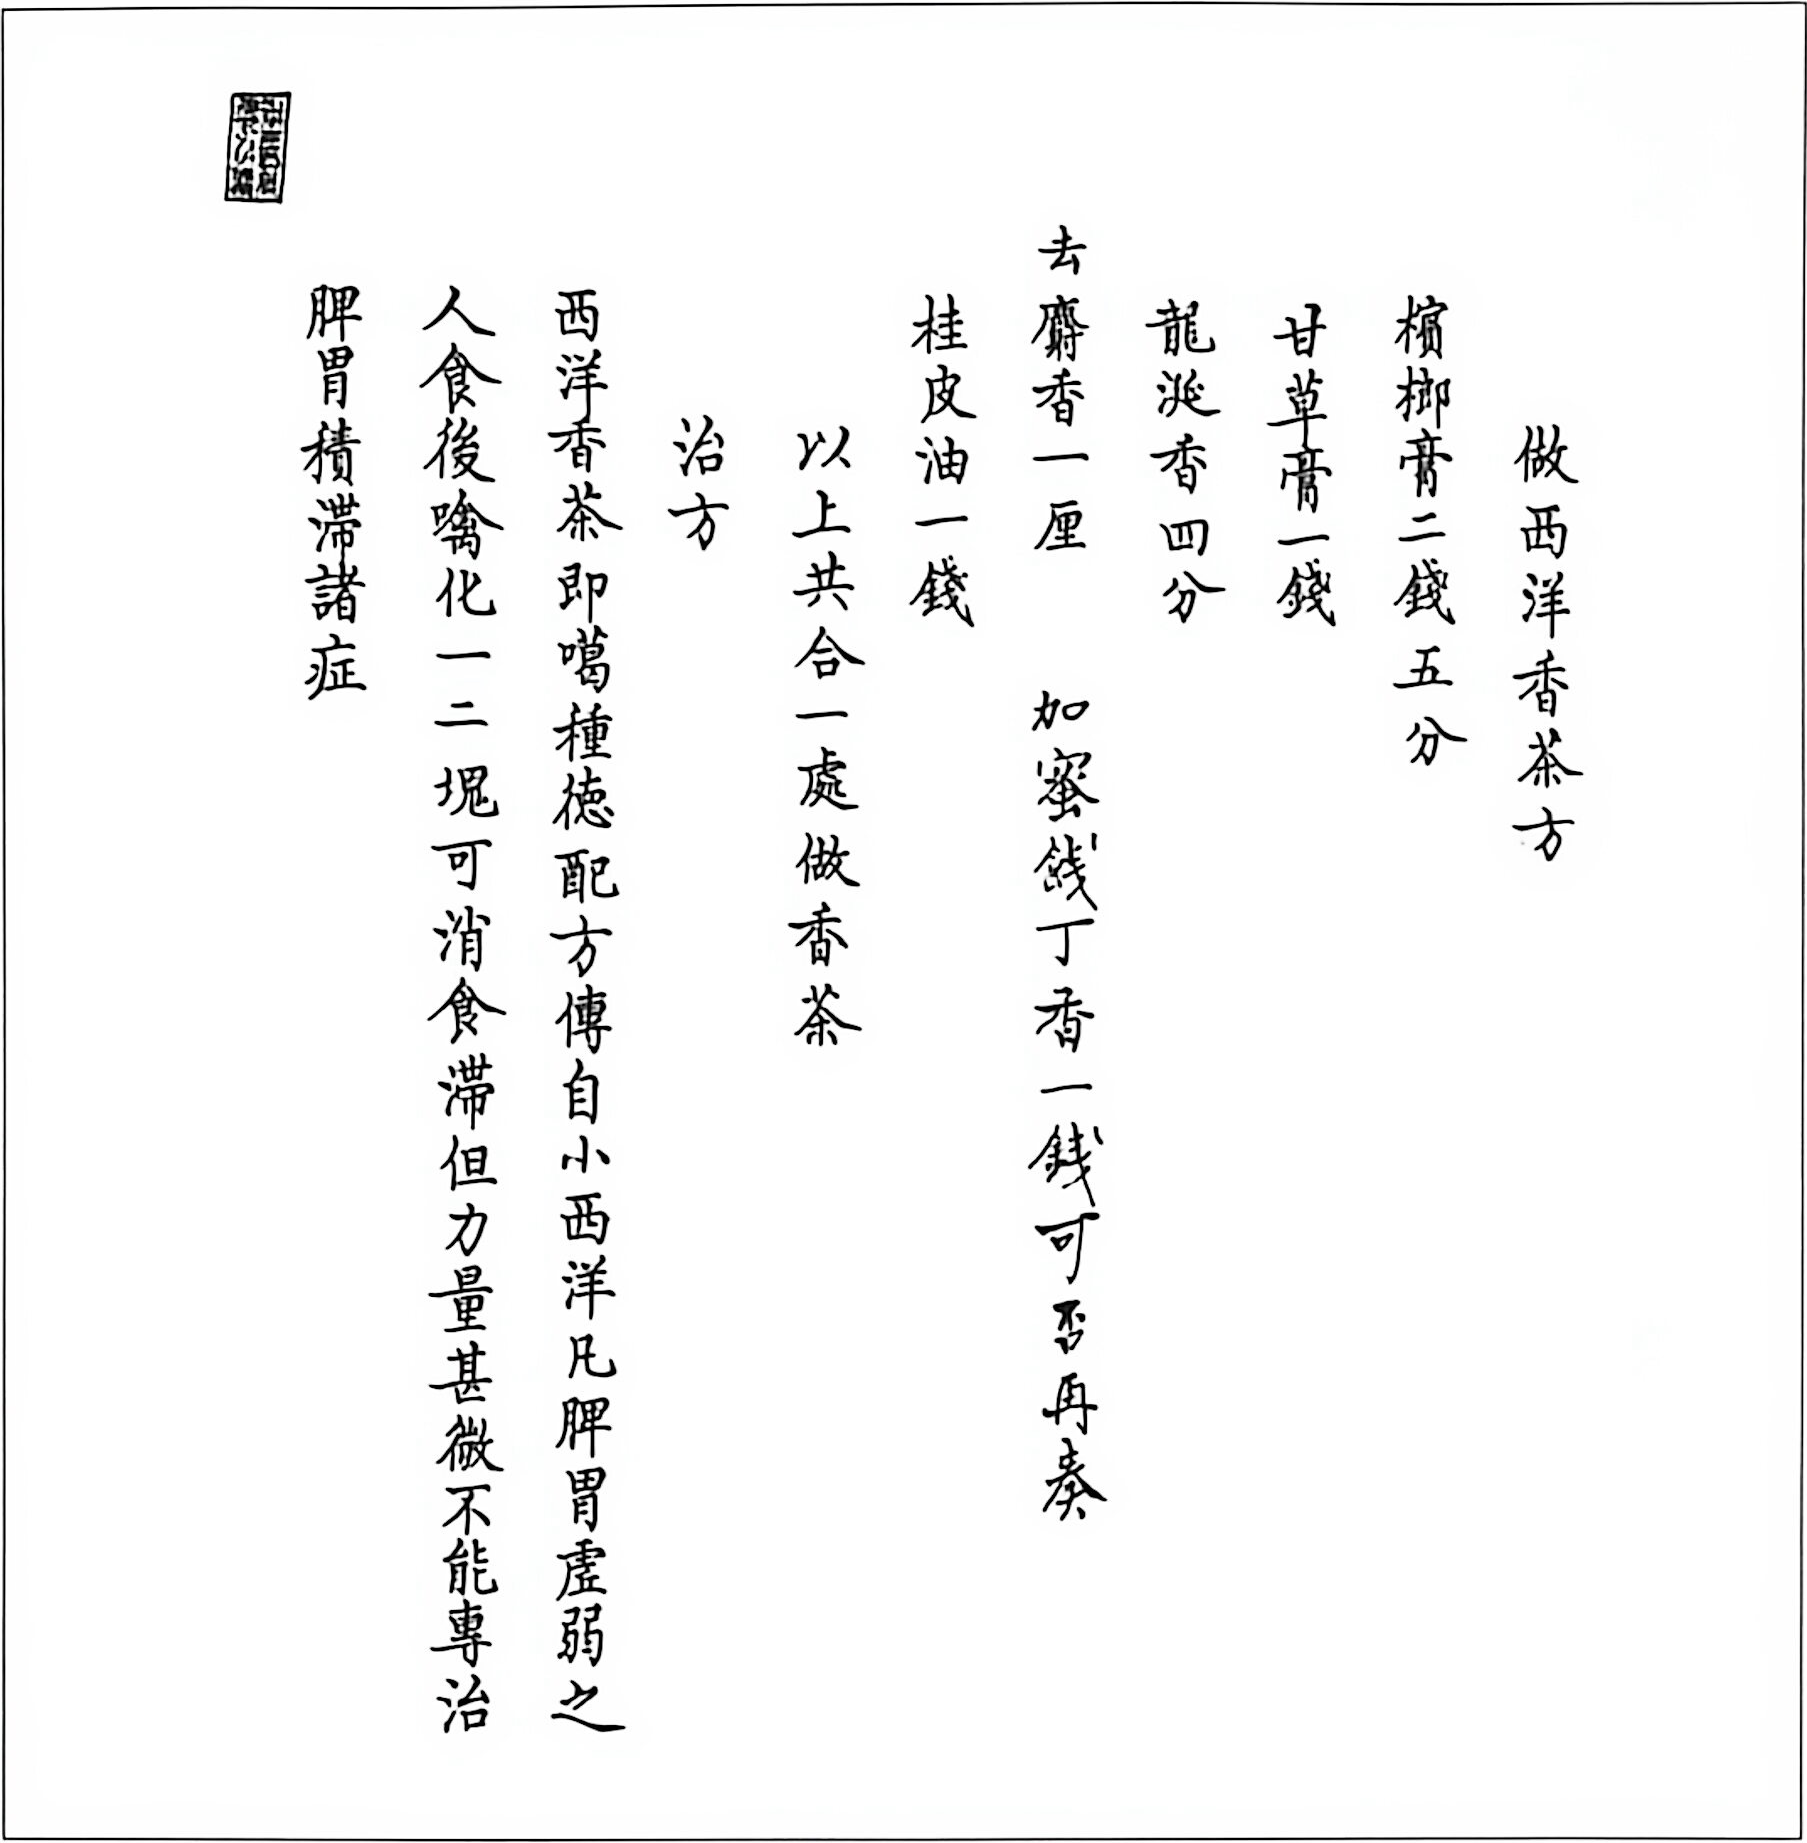
\includegraphics[width=\linewidth,height=.76\textheight,keepaspectratio]{assets/figures/tournon-prescription.png}
\caption*{图4.4\quad 故宫档案藏治疗教皇使节多罗药方}
\BookFloatNotes{图片来源：冯明珠，《坚持与容忍——档案中所见康熙皇帝对中梵关系生变的因应》，182。}
\end{figure}%
示感谢。还有一次，宫里一位西洋画家，大约是画画时间太久，肩%
痛难忍，康熙派医生过去，医生报告说最好的治疗方法是用针灸，%
但是画家很害怕针灸，问康熙该怎么处理。\NoteRef{4}{66}传教士安多病了，康%
熙的御医去看诊，给出的诊断是“中气不足，脾胃虚损，四肢厥冷，%
大便溏稀”等等，开出的是以“附子、干姜、白术”等组成的理中%
汤（是附子理中汤加减）。本来这个病症配搭这个药方是中医的标准%
治法，但有意思的是，御医还加了一句“其病情重大”，可以再用一%
些“圣药德里雅噶”。\NoteRef{4}{67}这个德里雅噶是Theriac的音译，这是古希腊%
开始就有的西药，主要是解毒之用，一直流行到19世纪。\NoteRef{4}{68}传教士%
人华后，把德里雅噶介绍给康熙，并帮助制作出来，存在宫里。康%
熙的御医应该用过这个药，所以才会给安多开出理中汤和德里雅噶%
并用的药方。\NoteRef{4}{69}康熙内廷中备有许多传教士介绍过来的药，这些药当%
时被称为“圣药”，即皇帝才有的药。这些“圣药”不仅宫里人知道，%
康熙私人圈子里的人也都知道。下面一段是康熙在江南的包衣奴才%
李煦去扬州探望病中的曹寅后，向康熙汇报了曹寅的病情，并求“圣%
药”治病的奏折：%
\par
% 原书页码：147；段落
{\bookkai 臣李煦跪奏：江宁织造臣曹寅于六月十六日自江宁来至扬州书局}%
{\bookkai 料理刻工，于七月初一日感受风寒，卧病数日，转而成疟，虽服药调}%
{\bookkai 理，日渐虚弱。……臣随于十五日亲至扬州看视。曹寅向臣言：我病}%
{\bookkai 时来时去，医生用药不能见效，必得主子圣药救我。但我儿子年小，}%
{\bookkai 今若打发他求主子去，目下我身边又无看视之人。求你替我启奏，如}%
{\bookkai 同我自己一样。若得赐药，则尚可起死回生，实蒙天恩再造等语。}%
\par
% 原书页码：147；段落
{\bookkai 臣今在扬看其调理，但病势甚重，臣不敢不据实奏闻，伏乞睿鉴。}%
\par
% 原书页码：147；段落
这里曹寅求的“圣药”就是治疗疟疾的金鸡纳树皮。从下面康熙的回%
复中，可以看出康熙当年被治好后，还仔细研究过传统中医治疗疟疾%
中可能存在的问题，以及金鸡纳这种药的使用注意事项：%
\par
% 原书页码：148；段落
{\bookkai 朱批：尔奏得好。今欲赐治疟疾的药，恐迟延，所以赐驿马星夜赶}%
{\bookkai 去。但疟疾若未转泄痢，还无妨。若转了病，此药用不得。南方庸医，}%
{\bookkai 每每用补济，而伤人者不计其数，须要小心。曹寅元肯吃人参，今得此}%
{\bookkai 病，亦是人参中来的。金鸡拿专治疟疾。用二钱末酒调服。若轻了些，}%
{\bookkai 再吃一服。必要住的。住后或一钱，或八分。连吃二服。可以出根。若}%
% 注70：用户于2026-10-12核对纸书第148页，确认在末句“万嘱！”后、下段之前。
{\bookkai 不是疟疾，此药用不得，须要认真。万嘱，万嘱，万嘱，万嘱！}\NoteRef{4}{70}%
\par
% 原书页码：148；段落
康熙的四个“万嘱”也体现了他对曹寅的关心。在这之前，康熙就知%
道曹寅常吃人参，所以认为曹寅这次病恶化是补药吃错了的缘故。康%
熙的药还是去晚了，曹寅在药送到前去世了。从康熙与他亲近奴才的%
通信中，可看出康熙从实际出发，各种药物并用来治病的实例。在当%
时人眼中，“圣药”是皇帝那里才有的特效药，没有人在乎这药到底%
是中国的还是西洋的。%
\par
% 原书页码：148；段落
大部分传教士人华后，都被中国这片土地以及这里的人和文化所%
吸引，一生都没有再回过欧洲，并安葬在了中国。后来在乾隆朝出名%
的画家郎世宁，其实也是康熙朝人华的。康熙朝传教士愿意人华，跟%
传教士在华的地位分不开。他们是内务府的人，所谓“朝中有人好办%
事”，所以在地方上，他们也能得到各种照顾。这些客观条件，不仅%
方便了他们传教，也促使这些传教士深人地了解中国的方方面面，并%
介绍回欧洲。历史写作和阅读容易时空穿越，但理解历史需要站在当%
时的时空中来理解。在当时的时空中，并没有近代以来产生的所谓西%
方意味着先进和进步这样的观念。当时的中西交流就是相隔很远的两%
个不同文明区域在互通有无、互有启发地平等交流。%
% 原书页码：149；标题
\subsection{小结}
\par
% 原书页码：149；段落
大清的权力分布就是个金字塔，皇帝处于最顶端。当传教士能够%
接近处于塔尖的皇帝和王公大臣，他们就处在一个有利的位置。接近%
高层，接近满人权贵，从而为传教打开方便之门，是清初传教士的策%
略。他们希望以有限的人手撬动大清这个幅员广阔、人口众多的国家，%
最大程度把他们的福音传到中国。南怀仁为如何实现这个基本目标指%
明了方向：就是要像包衣奴才一样与皇帝和满人权贵建立关系。这改%
变了汤若望和之前明代人华传教士希望通过在朝廷做大臣来接触皇帝%
的策略。南怀仁的策略调整反映了他对大清权力结构的深刻了解。大%
清的权力系统有两个：一个是从明代那里继承下来的基于君臣关系的%
朝廷系统；另外一个是满人的内部系统，其中康熙和他的部下讲的是%
主奴关系。%
\par
% 原书页码：149；段落
主奴关系及其衍生出来的派系是理解清初政治的核心。朝廷各部，%
人员流动及升迁任用，表面上看讲的是资历，但真正在后面起关键作%
用的是人员的派系。而这个派系和八旗里面基于主奴关系产生出来的%
派系有关。传教士是看明白了这一点的，所以后来的传教士到北京以%
后，都专注于进人内务府，私下为皇帝服务，争取像满人奴才一样获%
得皇帝的信任。%
\par
% 原书页码：149–150；段落（跨页续段）
维系清初皇亲国戚私人圈子的纽带是信任。这和官僚系统不一样。%
官僚系统通过科举吸收新人，其核心是才能。在私人圈子中，“信任”%
的来源有二：一是来自各种世袭关系，其中最主要的是血缘、姻亲以%
及主奴三种世袭关系；第二个来源是保荐。圈中的人把外面的人推荐%
到圈子中来，这个推荐人其实是用他在圈中已获得的信任来担保新人。%
（见下图）%
\par
% 原书页码：150–151；段落（跨页续段）
传教士能在鳌拜时期就进人康熙的内部圈子，信任来自于主奴关%
系。有了信任，传教士才能被纳人圈子中，开始了和康熙的往来。在%
往来过程中，双方关系变近，传教士就有了特权。这些特权包括可以%
私下见到康熙，有专门和康熙联系的通讯渠道，以及在地方上获得优%
% 原书页码：150；图表（图题／表题所在页）
\begin{figure}[tbp]
\centering
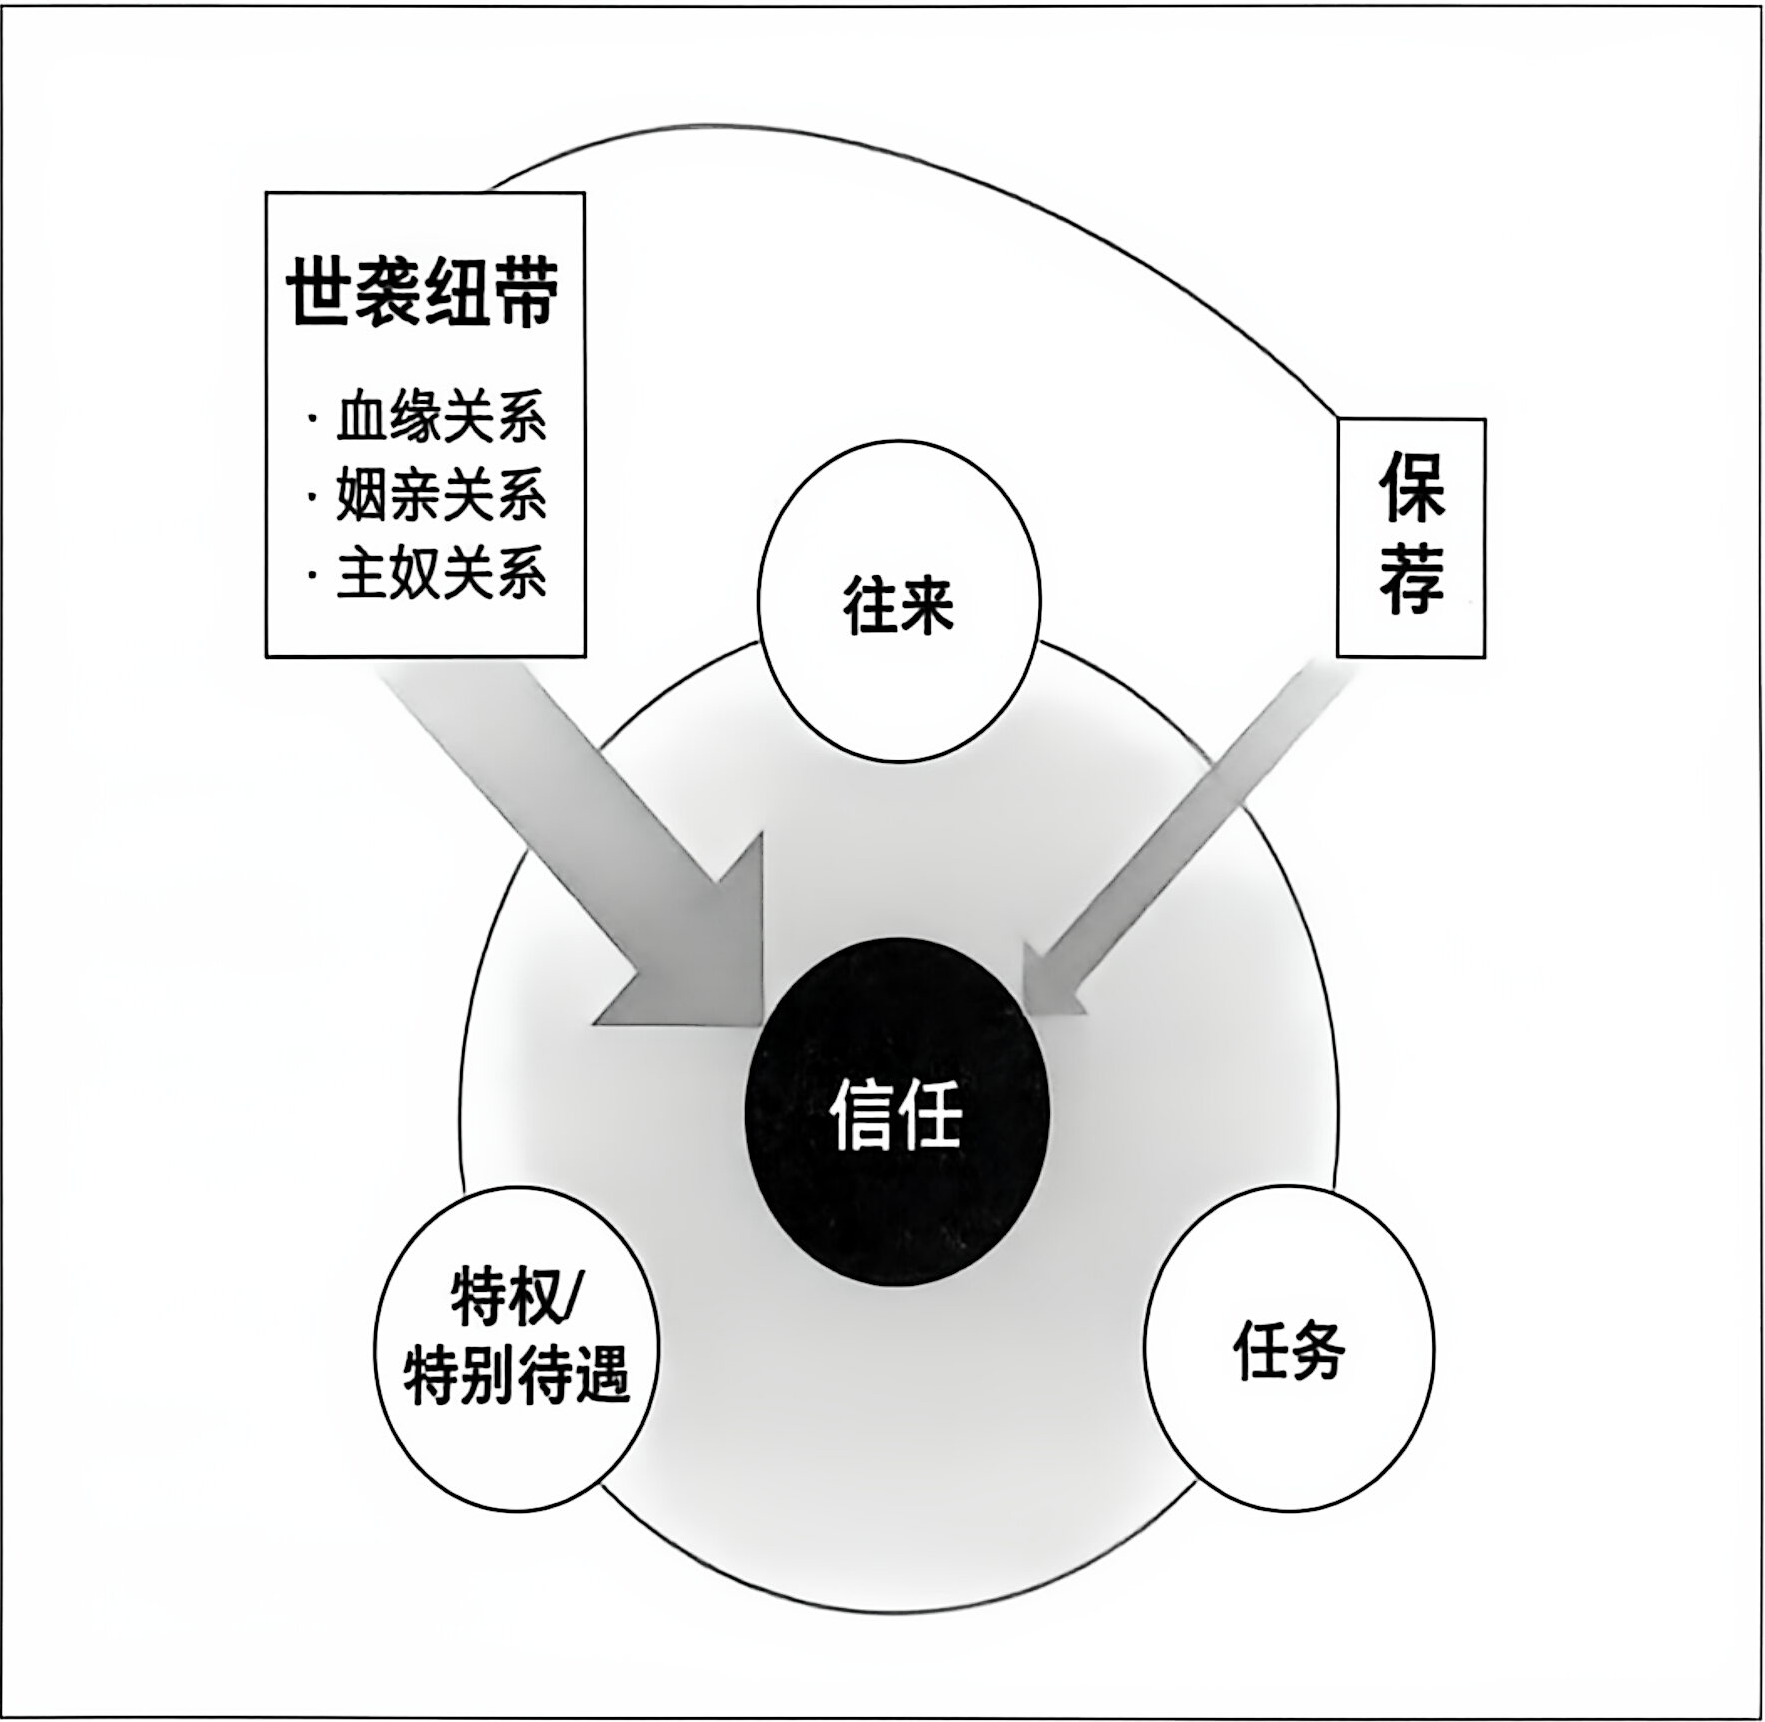
\includegraphics[width=\linewidth,height=.76\textheight,keepaspectratio]{assets/figures/kangxi-private-network.png}
\caption*{康熙私人关系网络运行示意图}
\end{figure}%
待，等等。有了这些特权，也便于传教士完成康熙分配的任务。在完%
成一个个任务的过程中又加强了双方的往来和信任。这就形成了一个%
良性循环。这三个要素的循环在清初以来的私人关系网中随处可见，%
而整个过程中最核心的就是信任。只要信任没有因为某件大事被破坏，%
那么双方关系就会持续。所幸的是，传教士在康熙一朝都没有辜负康%
熙对他们的信任，包括后来教皇派使节到中国来的时候。%
\par
% 原书页码：151；段落
康熙把传教士纳入自已私人圈子，其实也方便他对传教士的管%
理和任用。从皇帝的权力运作方面来讲，大清从明代那里继承下来%
的朝廷制度有很多条条框框。康熙作为皇帝，也必须尊重这些朝廷%
规矩，不能不理会大臣们的意见。容教诏书通过的全过程就很能说%
明问题。当时传教士就在写给欧洲信中解释过：“当皇帝征求大臣们%
的意见时，大臣们根据国法来回答，人们既不能责备他们，也不能%
对他们进行任何非难。”\NoteRef{4}{71}所以，最后康熙解决问题的方法还是派索额%
图去私下活动疏通。由于有朝廷的规章制度在，后来康熙和传教士%
都在有意识地避免把问题送到朝廷的官僚体系下去解决。对于康熙%
来说，绕开朝廷的方法就是把问题变成家事，这样就可以顺理成章%
地让内务府来处理。内务府就是康熙的内府，里面的事就是他的家%
事，自然里面的一切都是康熙一个人说了算，这样他就完全不需要%
考虑朝廷那边的各种成规。康熙如何把“国事”操办成“家事”，这%
就是后面两章的话题。%
